%% berlin_day-1.tex
%% Berlin Causal Inference Workshop — Day 1
%% 2×2, Parallel Trends, Event Studies, Covariates
%% Scott Cunningham · Baylor University
%%
%% Target: 48 slides, 90 minutes (10:00–11:30)
%% Compile: pdflatex berlin_day-1.tex

\documentclass[aspectratio=169,11pt]{beamer}
\usepackage{remix}
\usepackage{kuleuven_theme}

\usepackage{tikz}
\usetikzlibrary{positioning,arrows.meta,calc,shapes.geometric,fit,backgrounds}
\usepackage{listings}
\usepackage{xcolor}
\usepackage{booktabs}
\usepackage{colortbl}
\usepackage{amsmath}

%% ---------- Sandwich-estimator color tracing (bread / meat) ----------
\definecolor{breadcolor}{HTML}{2B6CB0}
\definecolor{meatcolor}{HTML}{A51C30}
\newcommand{\bread}[1]{\textcolor{breadcolor}{#1}}
\newcommand{\meat}[1]{\textcolor{meatcolor}{#1}}

%% ---------- TikZ styles ----------
\tikzset{
  ingredient/.style={
    rectangle, rounded corners=2pt, draw=accent, line width=0.8pt,
    fill=cream, text=charcoal, font=\bfseries,
    minimum width=4.8cm, minimum height=1.6cm, align=center
  },
  cell/.style={
    rectangle, draw=charcoal, line width=0.5pt,
    fill=lightbg, text=charcoal,
    minimum width=3.0cm, minimum height=1.3cm, align=center, font=\small
  },
  celltreated/.style={
    rectangle, draw=accent, line width=1.2pt,
    fill=remixgreenlight, text=charcoal,
    minimum width=3.0cm, minimum height=1.3cm, align=center, font=\small
  },
  trendline/.style={line width=1pt, accent},
  trendcontrol/.style={line width=1pt, slate, dashed},
}

%% ---------- listings ----------
\lstset{
  basicstyle=\ttfamily\footnotesize,
  keywordstyle=\color{accentdark}\bfseries,
  commentstyle=\color{warmgray}\itshape,
  stringstyle=\color{ocean},
  backgroundcolor=\color{lightbg},
  frame=single, framesep=4pt,
  rulecolor=\color{warmgray!40},
  columns=fullflexible,
  showstringspaces=false,
  breaklines=true,
  numbers=none,
  xleftmargin=0.4em, xrightmargin=0.4em,
}

%% ---------- counterfactual maroon ----------
\definecolor{maroon}{HTML}{7A0C0C}

%% ---------- emphbox ----------
\newcommand{\emphbox}[1]{%
  \begin{beamercolorbox}[rounded=true,sep=7pt,wd=\linewidth]{block body}%
    \small\color{slate}\raggedright #1%
  \end{beamercolorbox}}

\begin{document}

%% ============================================================
%% TITLE
%% ============================================================

\codechellatitle
  {Foundations of Difference-in-Differences}
  {The 2$\times$2 and Parallel Trends}
  {Scott Cunningham \textperiodcentered\ Baylor University}
  {KU Leuven \textperiodcentered\ Difference-in-Differences Workshop}

\begin{frame}{About me}
\vspace{0.4em}
\begin{itemize}\setlength\itemsep{0.6em}
  \item \highlight{Scott Cunningham} --- Professor of Economics, Baylor University; Visiting Professor of Government, Harvard University.
  \item This is a \highlight{3-day workshop on difference-in-differences} --- from the basic 2$\times$2 through continuous treatment and staggered adoption.
  \item Much of the material is drawn from \highlight{Baker, Callaway, Cunningham, Goodman-Bacon \& Sant'Anna (2026)}, ``Difference-in-Differences: A Practitioner's Guide,'' \textit{Journal of Economic Literature}, and new work on continuous-treatment DiD.
\end{itemize}
\end{frame}

\begin{frame}{Three days}
\vspace{0.4em}
\begin{center}
\renewcommand{\arraystretch}{1.6}
\small
\begin{tabular}{@{}llp{6.8cm}@{}}
\toprule
\textbf{Day} & \textbf{Time} & \textbf{Topic} \\
\midrule
Day 1 & 10:00--11:30am & 2$\times$2 DiD: parameters, calculations, identification, covariates \\
Day 2 & 9:00--10:30am  & Continuous treatment DiD \\
Day 3 & 11:00am--12:30pm & Staggered adoption DiD \\
\bottomrule
\end{tabular}
\end{center}
\end{frame}

\begin{frame}{Today: from the 2$\times$2 to covariates}
\vspace{0.4em}
\begin{itemize}\setlength\itemsep{0.5em}
  \item What the 2$\times$2 DiD is --- as a \highlight{calculation} and as an \highlight{identification strategy}.
  \item Six equivalent ways to compute the 2$\times$2 --- and why that matters.
  \item What the DiD actually identifies: ATT under parallel trends.
  \item Event studies --- what they tell you and what they don't.
  \item When covariates are needed and how to include them correctly.
\end{itemize}
\end{frame}

%% ============================================================
%% PART 1. DiD = TWO THINGS
%% ============================================================
\remixsection{DiD is Two Things: Calculation + Assumption}

\begin{frame}[shrink=8]{DiD is a research design, not a regression}
\vspace{0.6em}
\pullquote{A research design is an identification strategy: it reveals the invisible target parameter hidden inside a calculation.}{}
\vspace{0.6em}
\begin{center}
\begin{tikzpicture}
\node[ingredient] (calc) at (-3.2,0) {%
  \textcolor{accent}{\large 1.} \\[0.3em]
  A \textit{calculation}\\[0.2em]
  \scriptsize\textcolor{warmgray}{(the 2$\times$2)}
};
\node[ingredient] (assn) at (3.2,0) {%
  \textcolor{accent}{\large 2.} \\[0.3em]
  An \textit{assumption}\\[0.2em]
  \scriptsize\textcolor{warmgray}{(parallel trends)}
};
\node[font=\Large\bfseries,text=accent] at (0,0) {+};
\end{tikzpicture}
\end{center}
\end{frame}

\begin{frame}{The individual treatment effect}
\vspace{1.2em}
\begin{center}
\Large
\[
\delta_i \;=\; Y_i(1) - Y_i(0)
\]
\end{center}
\vspace{0.6em}
\begin{itemize}
  \item One per unit. \highlight{Different} across units in general --- treatment effects are heterogeneous.
  \item We only ever see one of $Y_i(1)$ or $Y_i(0)$. The other is the counterfactual.
  \item So $\delta_i$ is never directly observed at the individual level.
\end{itemize}
\end{frame}

\begin{frame}{The ATT: a causal parameter has three ingredients}
\vspace{1.4em}
\begin{center}
\Large
\[
\text{ATT} \;=\; \underbrace{\mathbb{E}\big[\,}_{\text{\normalsize \color{accent} weighted expectations}}\;
\underbrace{Y(1) - Y(0)}_{\text{\normalsize \color{accent} potential outcomes}}\;
\underbrace{\big|\; D = 1,\,\text{Post}\,\big]}_{\text{\normalsize \color{accent} population}}
\]
\end{center}
\vspace{1.4em}
\begin{itemize}
  \item \highlight{Potential outcomes} --- the contrast $Y(1) - Y(0)$
  \item \highlight{Population} --- on whom: treated units, post-period
  \item \highlight{Weighted expectations} --- how we average across that population
\end{itemize}
\end{frame}

\begin{frame}{The switching equation: you see one half}
\vspace{0.8em}
\begin{center}
\Large
\[
Y_i \;=\; D_i \cdot Y_i(1) \;+\; (1 - D_i) \cdot Y_i(0)
\]
\end{center}
\vspace{1em}
\begin{itemize}\setlength\itemsep{6pt}
  \item For each unit: $Y_i(1)$ if treated, $Y_i(0)$ if not.
  \item The ATT asks about \textit{both} columns. The data hands you one.
\end{itemize}
\vspace{0.8em}
\meta{The rest of today: strategies for recovering the ATT from the half we see.}
\end{frame}

%% ============================================================
%% PART 2. SIX EQUIVALENT WAYS, ONE NUMBER
%% ============================================================
\remixsection{Six Equivalent Ways, One Number}

\begin{frame}[shrink=6]{Cheng \& Hoekstra (2013): castle doctrine and homicide}
\vspace{0.2em}
\footnotesize
\textbf{The reform.} ``Castle doctrine'' laws expanded the legal right to use lethal force in self-defense. Many US states passed expansions from \highlight{2005--2010}.
\vspace{0.2em}
\begin{itemize}
  \item \textbf{Panel:} all US states $\times$ years. \textbf{Outcome:} log homicide rate.
  \item \textbf{Treatment:} state passed a castle doctrine expansion.
  \item \textbf{Comparison:} states that did not pass (never-treated).
\end{itemize}
\vspace{0.4em}
For today: a clean 2$\times$2 on \highlight{2005--2006}. Treated $=$ states adopting in 2006; control $=$ states that hadn't.
\vspace{0.4em}
\meta{Cheng \& Hoekstra (2013), \textit{J. Human Resources} 48(3): 821--854.}
\end{frame}

\begin{frame}[fragile]{The four cells, by hand on \texttt{castle.dta}}
\vspace{0.2em}
\begin{lstlisting}[language={[ANSI]C}]
use castle.dta, clear
keep if year >= 2005 & year <= 2006
gen post  = (year == 2006)
gen treat = (effyear == 2006)

summarize l_homicide if treat==1 & post==1   // Y11
summarize l_homicide if treat==1 & post==0   // Y10
summarize l_homicide if treat==0 & post==1   // Y01
summarize l_homicide if treat==0 & post==0   // Y00
\end{lstlisting}
\vspace{0.4em}
\begin{center}
\small
$\widehat{\text{DiD}} = (\overline{Y}_{11} - \overline{Y}_{10}) - (\overline{Y}_{01} - \overline{Y}_{00}) \;\approx\; \mathbf{0.10}$
\end{center}
\begin{center}
\small\color{warmgray}\itshape Log homicide rate $\sim 10\%$ higher in 2006-adopting states relative to non-adopters.
\end{center}
\end{frame}

\begin{frame}{Four averages, three subtractions --- two orderings}
\vspace{0.2em}
\small
The 2$\times$2 is four cell means: $\;\overline{Y}_{11},\;\overline{Y}_{10},\;\overline{Y}_{01},\;\overline{Y}_{00}$.
\vspace{0.4em}
\begin{columns}[T]
\column{0.47\textwidth}
\textbf{First-difference ordering ($\rightarrow$)}\\[0.4em]
Subtract across time \textit{within} each group, then compare groups:
\begin{align*}
\Delta_1 &= \overline{Y}_{11} - \overline{Y}_{10} \\
\Delta_0 &= \overline{Y}_{01} - \overline{Y}_{00} \\[2pt]
\text{DiD} &= \Delta_1 - \Delta_0
\end{align*}

\column{0.47\textwidth}
\textbf{Group-difference ordering ($\downarrow$)}\\[0.4em]
Subtract across groups \textit{within} each period, then compare periods:
\begin{align*}
G_{\text{post}} &= \overline{Y}_{11} - \overline{Y}_{01} \\
G_{\text{pre}}  &= \overline{Y}_{10} - \overline{Y}_{00} \\[2pt]
\text{DiD} &= G_{\text{post}} - G_{\text{pre}}
\end{align*}
\end{columns}
\vspace{0.3em}
\emphbox{Same four averages. Same three subtractions. Same number. The 2$\times$2 is symmetric under reordering.}
\end{frame}

\begin{frame}{Six equivalent ways, one number}
\vspace{0.2em}
\begin{center}
\renewcommand{\arraystretch}{1.35}
\footnotesize
\begin{tabular}{@{}clcc@{}}
\toprule
 & \textbf{Way} & \textbf{What it does} & \textbf{$\hat\beta_{DD}$} \\
\midrule
1. & First-difference arithmetic & $(\overline{Y}_{11}-\overline{Y}_{10})-(\overline{Y}_{01}-\overline{Y}_{00})$ & \highlight{$\approx 0.10$} \\
2. & Group-difference arithmetic & $(\overline{Y}_{11}-\overline{Y}_{01})-(\overline{Y}_{10}-\overline{Y}_{00})$ & \highlight{$\approx 0.10$} \\
\midrule
3. & OLS with \texttt{post\#\#treat} & saturated dummies, direct interaction & \highlight{$\approx 0.10$} \\
4. & Two-way fixed effects (TWFE) & absorbs unit $+$ time means & \highlight{$\approx 0.10$} \\
5. & $\Delta Y_i$ on $D_i$ (horizontal) & time-difference within group, then on $D$ & \highlight{$\approx 0.10$} \\
6. & $G_t$ on $\text{Post}_t$ (vertical) & group-difference within period, then on Post & \highlight{$\approx 0.10$} \\
\bottomrule
\end{tabular}
\end{center}
\vspace{0.3em}
\begin{center}
\small\color{warmgray}\itshape
Same data, six ways, identical to machine epsilon.
\end{center}
\end{frame}

\begin{frame}{``DiD'' is not a regression --- there are six equivalent ways to compute it}
\vspace{0.4em}
\begin{itemize}\setlength\itemsep{0.5em}
  \item You will often hear: ``I ran a diff-in-diff regression.''
  \item That is misleading. Two of the six ways are pure arithmetic; four are regressions. All give the same answer.
  \item The regressions are tools for requesting the estimate. The \highlight{2$\times$2 is the thing being estimated}.
\end{itemize}
\vspace{0.4em}
\emphbox{This is why we start with the 2$\times$2, not the regression. The estimand is four averages and three subtractions. The regression is just a convenient way to compute --- and standard-error --- it.}
\end{frame}

%% ============================================================
%% PART 3. DECOMPOSING THE 2×2
%% ============================================================
\remixsection{Decomposing the 2$\times$2}

\begin{frame}{The proof: add a zero, rearrange (four steps)}
\vspace{-0.3em}
\footnotesize

\textbf{1.\ Start with the 2$\times$2:}
\vspace{-0.4em}
\[
\widehat{\text{DiD}} \;=\; \big[\mathbb{E}[Y\mid 1,\text{Post}] - \mathbb{E}[Y\mid 1,\text{Pre}]\big]
                    \;-\; \big[\mathbb{E}[Y\mid 0,\text{Post}] - \mathbb{E}[Y\mid 0,\text{Pre}]\big]
\]
\vspace{-0.8em}

\textbf{2.\ Switching equation.}\;Treated-post is $Y(1)$; the other three cells are $Y(0)$:
\vspace{-0.4em}
\[
\widehat{\text{DiD}} \;=\; \big[\mathbb{E}[Y(1)\mid 1,\text{Post}] - \mathbb{E}[Y(0)\mid 1,\text{Pre}]\big]
                    \;-\; \big[\mathbb{E}[Y(0)\mid 0,\text{Post}] - \mathbb{E}[Y(0)\mid 0,\text{Pre}]\big]
\]
\vspace{-0.6em}

\textbf{3.\ Add a zero.}\;Insert
${\color{maroon}+\,\mathbb{E}[Y(0)\mid 1,\text{Post}] - \mathbb{E}[Y(0)\mid 1,\text{Post}]}$
(the missing counterfactual, twice):
\vspace{-0.3em}
\begin{align*}
\widehat{\text{DiD}} \;=\;&\;
  \mathbb{E}[Y(1)\mid 1,\text{Post}]
  {\color{maroon}\;-\;\mathbb{E}[Y(0)\mid 1,\text{Post}]} \\[-2pt]
&\;{\color{maroon}+\;\mathbb{E}[Y(0)\mid 1,\text{Post}]}
  - \mathbb{E}[Y(0)\mid 1,\text{Pre}]
  \;-\;\big[\mathbb{E}[Y(0)\mid 0,\text{Post}] - \mathbb{E}[Y(0)\mid 0,\text{Pre}]\big]
\end{align*}
\vspace{-0.6em}

\textbf{4.\ Rearrange.}\;First two terms $=$ ATT; remainder $=$ difference in untreated trends:
\vspace{-0.4em}
\[
\widehat{\text{DiD}} \;=\;
  \underbrace{\mathbb{E}\!\big[Y(1){\color{maroon}-Y(0)}\mid 1,\text{Post}\big]}_{\textstyle\text{\color{accent}\bfseries ATT}}
  \;+\;
  \underbrace{{\color{maroon}\Delta\mathbb{E}[Y(0)\mid 1]} \;-\; \Delta\mathbb{E}[Y(0)\mid 0]}_{\text{PT bias} \;=\; 0 \text{ under parallel trends}}
\]
\end{frame}

\begin{frame}{The bias term \textit{is} selection bias --- on trends, not levels}
\footnotesize
\[
\text{bias} \;=\; \underbrace{\Delta\mathbb{E}[Y(0)\mid D{=}1]}_{\text{how treated's $Y(0)$ moves}} \;-\; \underbrace{\Delta\mathbb{E}[Y(0)\mid D{=}0]}_{\text{how controls' $Y(0)$ moves}}
\]
\begin{itemize}
  \item \textbf{Cross-section selection bias}: are treated and control different in \textit{levels} of $Y(0)$?
  \item \textbf{DiD's selection bias}: are treated and control different in \textit{trends} of $Y(0)$?
  \item Different levels are fine --- unit fixed effects absorb them.
  \item What can't differ is the \textit{rate} at which $Y(0)$ moves across groups.
\end{itemize}
\begin{block}{The trade DiD makes vs.\ randomization}
RCTs guarantee identical trends (and levels) through the design itself. \\
DiD requires only one thing: parallel trends in $Y(0)$. But unlike randomization, \highlight{there is no guaranteed research design that delivers it} --- it must be argued for on substantive grounds.
\end{block}
\meta{Ghanem, Sant'Anna \& W\"{u}thrich (2025).}
\end{frame}

\begin{frame}{Case 2: no-anticipation fails --- treated group adjusts early}
\footnotesize
Treated units \textit{anticipate} the policy and adjust before it lands. Their pre-period outcome is contaminated:
\[
\mathbb{E}[Y\mid 1,\text{Pre}] \;=\; \mathbb{E}[Y(0)\mid 1,\text{Pre}] \;+\; \textcolor{accent}{\text{ATT}_{\text{pre}}}
\]
\vspace{-0.3em}
Apply the same $+0$ trick as Case 1. The contaminated pre-period subtracts off:
\[
\widehat{\text{DiD}} \;=\;
  \underbrace{\text{ATT}_{\text{Post}}}_{\text{what we want}}
  \;+\; \underbrace{\Delta\mathbb{E}[Y(0)\mid 1] - \Delta\mathbb{E}[Y(0)\mid 0]}_{\text{PT bias}\;=\;0}
  \;-\; \underbrace{\textcolor{accent}{\text{ATT}_{\text{pre}}}}_{\text{anticipation bias}}
\]
\vspace{-0.2em}
\begin{block}{Numerical example}
ATT $= 10$, PT bias $= 0$, ATT$_{\text{pre}} = 3$.
\quad $\widehat{\text{DiD}} = 10 - 3 = \mathbf{7}$. \;\highlight{Biased down.}
\end{block}
\meta{If effects are constant over time, ATT$_{\text{pre}} =$ ATT$_{\text{post}}$ and DiD $\to 0$.}
\end{frame}

\begin{frame}{Case 3: SUTVA fails --- control group is also treated in Post}
\footnotesize
The comparison group's Post outcome is $Y(1)$, not $Y(0)$ (spillover or simultaneous treatment):
\[
\widehat{\text{DiD}} \;=\; \big[\mathbb{E}[Y(1)\mid 1,\text{Post}] - \mathbb{E}[Y(0)\mid 1,\text{Pre}]\big]
                    \;-\; \big[\textcolor{accent}{\mathbb{E}[Y(1)\mid 0,\text{Post}]} - \mathbb{E}[Y(0)\mid 0,\text{Pre}]\big]
\]
\vspace{-0.3em}
Add \textit{two} zeros (one counterfactual on each side) and rearrange:
\[
\widehat{\text{DiD}} \;=\;
  \underbrace{\text{ATT}}_{\text{treated}}
  \;+\; \underbrace{\Delta\mathbb{E}[Y(0)\mid 1] - \Delta\mathbb{E}[Y(0)\mid 0]}_{\text{PT bias}\;=\;0}
  \;-\; \underbrace{\textcolor{accent}{\text{ATT}_{D{=}0,\,\text{Post}}}}_{\text{control's treatment effect}}
\]
\vspace{-0.2em}
\begin{block}{Numerical example}
ATT $= 10$, PT bias $= 0$, ATT$_{D{=}0,\text{Post}} = 4$.
\quad $\widehat{\text{DiD}} = 10 - 4 = \mathbf{6}$. \;\highlight{Biased toward zero.}
\end{block}
\end{frame}

\begin{frame}{Case 4: comparison group is always treated}
\footnotesize
The comparison group was treated \textit{before} our data starts. Both their Pre and Post outcomes are $Y(1)$:
\[
\widehat{\text{DiD}} \;=\; \big[\mathbb{E}[Y(1)\mid 1,\text{Post}] - \mathbb{E}[Y(0)\mid 1,\text{Pre}]\big]
                    \;-\; \big[\textcolor{accent}{\mathbb{E}[Y(1)\mid 0,\text{Post}] - \mathbb{E}[Y(1)\mid 0,\text{Pre}]}\big]
\]
\vspace{-0.3em}
Add $\pm\mathbb{E}[Y(0)\mid 0,\text{Post}]$ and $\pm\mathbb{E}[Y(0)\mid 0,\text{Pre}]$ on the comparison side and rearrange:
\[
\widehat{\text{DiD}} \;=\;
  \underbrace{\text{ATT}}_{\text{treated}}
  \;+\; \underbrace{\Delta\mathbb{E}[Y(0)\mid 1] - \Delta\mathbb{E}[Y(0)\mid 0]}_{\text{PT bias}\;=\;0}
  \;-\; \underbrace{\textcolor{accent}{\Delta\,\text{ATT}_{D{=}0}}}_{\text{change in comparison's TE}}
\]
\vspace{-0.2em}
\begin{block}{Numerical example}
ATT $= 10$, PT bias $= 0$, $\Delta$ATT$_{D{=}0} = 2$.
\quad $\widehat{\text{DiD}} = 10 - 2 = \mathbf{8}$. \;\highlight{Biased toward zero.}
\end{block}
\end{frame}

\begin{frame}{Four cases: one method}
\vspace{0.2em}
\small
\renewcommand{\arraystretch}{1.55}
\begin{center}
\begin{tabular}{@{}lp{3.5cm}l@{}}
\toprule
\textbf{Case} & \textbf{What fails} & \textbf{$\widehat{\text{DiD}}\;=$} \\
\midrule
1. NA $+$ untreated comparison & nothing (baseline) & ATT $+$ PT bias \\
2. NA fails & treated Pre $\supset$ $Y(1)$ & ATT $+$ PT bias $-$ \textcolor{accent}{ATT$_{\text{pre}}$} \\
3. Spillover (SUTVA) & control Post $\supset$ $Y(1)$ & ATT $+$ PT bias $-$ \textcolor{accent}{ATT$_{D{=}0,\text{Post}}$} \\
4. Always-treated comparison & control Pre \& Post $\supset$ $Y(1)$ & ATT $+$ PT bias $-$ \textcolor{accent}{$\Delta$ATT$_{D{=}0}$} \\
\bottomrule
\end{tabular}
\end{center}
\vspace{0.4em}
\emphbox{Same method every time: write the 2$\times$2, apply the switching equation, add the right zero(s), rearrange. Only what you add changes.}
\end{frame}

\begin{frame}{New Jersey raises its minimum wage. Pennsylvania doesn't.}
\vspace{0.4em}
\begin{itemize}
  \item \highlight{April 1992}: NJ raises its minimum wage from \$4.25 to \$5.05 --- a 19\% increase.
  \item Pennsylvania, just over the river, stays at \$4.25.
  \item Card and Krueger survey 410 fast-food restaurants on both sides of the border, before (Feb 1992) and after (Nov 1992).
  \item The natural 2$\times$2: \highlight{treated $=$ NJ, control $=$ PA, pre/post the policy.}
\end{itemize}
\vspace{0.4em}
\meta{Card \& Krueger, \textit{American Economic Review}, 1994.}
\end{frame}

\begin{frame}{The 2$\times$2 as long differences: horizontal regression}
\vspace{0.2em}
\small
\textbf{Step 1:} Within each group, subtract across time (pre $\rightarrow$ post).
\vspace{0.4em}
\begin{center}
\renewcommand{\arraystretch}{1.5}
\begin{tabular}{@{}l rr r@{}}
\toprule
 & \textbf{Pre} & \textbf{Post} & \textbf{$\Delta$ ($\rightarrow$)} \\
\midrule
NJ (treated) & 20.44 & 21.03 & \textcolor{accent}{$+0.59$} \\
PA (control) & 23.33 & 21.17 & \textcolor{slate}{$-2.16$} \\
\bottomrule
\end{tabular}
\end{center}
\vspace{0.3em}
\textbf{Step 2:} Subtract the two time changes:
\[
  \widehat{\beta}_{\text{DiD}} \;=\; (+0.59) - (-2.16) \;=\; \highlight{+2.75}
\]
\vspace{0.1em}
\emphbox{Imbens: the \textbf{long-difference regression} (or \textbf{horizontal regression})\\[3pt]
$\Delta Y_i = \alpha + \beta_{\text{DiD}}\, D_i + u_i$\quad --- difference over time \textit{within} each group, then compare groups.}
\end{frame}

\begin{frame}{Parallel trends visualized: the control \textit{is} the counterfactual}
\vspace{0.1em}
\begin{center}
\begin{tikzpicture}[scale=1.0]
\draw[->, slate, thick] (0,0) -- (7.0,0) node[right, text=charcoal, font=\small] {time};
\draw[->, slate, thick] (0,0) -- (0,3.3) node[above, text=charcoal, font=\small] {employment};

\draw[dashed, warmgray] (3.0,0) -- (3.0,3.0);
\node[font=\scriptsize, text=warmgray, anchor=north] at (3.0,-0.1) {April 1992};

\draw[trendcontrol] (0.5,2.2) -- (5.5,1.6);
\draw[trendline] (0.5,1.4) -- (3.0,1.1);
\draw[trendline] (3.0,1.1) -- (5.5,1.25);
\draw[line width=0.8pt, accent, densely dotted] (3.0,1.1) -- (5.5,0.8);

\draw[<->, accent, line width=0.5pt] (5.7,0.8) -- (5.7,1.25);
\node[font=\scriptsize, text=accent, anchor=west] at (5.78,1.025) {2$\times$2 = ATT};

\node[font=\scriptsize, text=slate,  anchor=west] at (5.65,1.6) {PA $= Y(0)$};
\node[font=\scriptsize, text=accent, anchor=west] at (5.65,1.25) {NJ observed};
\node[font=\scriptsize, text=accent, anchor=west] at (5.65,0.65) {NJ $Y(0)$ counter.};
\end{tikzpicture}
\end{center}
\vspace{0.1em}
\begin{center}
\small\color{warmgray}\itshape
The dotted line is what NJ would have done absent the policy. \;We never see it. \\
\highlight{PT lets PA's slope stand in for it.}
\end{center}
\end{frame}

\begin{frame}{The same 2$\times$2 as group differences: vertical regression}
\vspace{0.1em}
\small
\textbf{Step 1:} At each time period, subtract across groups (NJ$-$PA, $\downarrow$).
\vspace{0.25em}
\begin{center}
\renewcommand{\arraystretch}{1.45}
\begin{tabular}{@{}l rr@{}}
\toprule
 & \textbf{Pre} & \textbf{Post} \\
\midrule
NJ (treated) & 20.44 & 21.03 \\
PA (control) & 23.33 & 21.17 \\
\midrule
\textbf{Gap (NJ$-$PA $\downarrow$)} & \textcolor{slate}{$-2.89$} & \textcolor{accent}{$-0.14$} \\
\bottomrule
\end{tabular}
\end{center}
\vspace{0.2em}
\textbf{Step 2:} Subtract the two group gaps:
\[
  \widehat{\beta}_{\text{DiD}} \;=\; (-0.14) - (-2.89) \;=\; \highlight{+2.75}
\]
\emphbox{Imbens: the \textbf{group-differences regression} (or \textbf{vertical regression})\\[3pt]
$D_t = \alpha + \beta_{\text{DiD}}\,\text{Post}_t + v_t$\quad --- compare groups \textit{within} each period, then difference across time.}
\end{frame}

\begin{frame}{Two orderings, one number --- and why the vertical view matters}
\vspace{0.2em}
\begin{center}
\renewcommand{\arraystretch}{1.45}
\small
\begin{tabular}{@{}lll@{}}
\toprule
\textbf{Ordering} & \textbf{Regression} & \textbf{Estimate} \\
\midrule
Time first, groups second ($\rightarrow$ then $\uparrow$) & Long-difference (horizontal) & $+2.75$ \\
Groups first, time second ($\downarrow$ then $\rightarrow$) & Group-differences (vertical) & $+2.75$ \\
\bottomrule
\end{tabular}
\end{center}
\vspace{0.4em}
\begin{itemize}\small
  \item Both orderings of the double-difference give the same number.
  \item The 2$\times$2 is symmetric under reordering --- it doesn't matter which subtraction comes first.
\end{itemize}
\vspace{0.2em}
\emphbox{\textbf{Why the vertical view matters (Imbens 2021):} Allow an intercept in the group-differences regression: $D_t = \mu + \beta_{\text{DiD}}\,\text{Post}_t$. That $\mu$ \textit{absorbs the level difference between the two groups} --- which is the key move in synthetic control. No convex-hull constraint required.}
\end{frame}

%% ============================================================
%% PART 5. STANDARD ERRORS (no section divider)
%% ============================================================

\begin{frame}[shrink=8]{Three flavors of standard error}
\vspace{0.4em}
\begin{itemize}
  \item \highlight{Vanilla (homoskedastic)}: assumes $\text{Var}(\varepsilon_i \mid X_i) = \sigma^2$ for all $i$.
  \item \highlight{Robust (HC)}: each residual speaks for itself --- handles heteroskedasticity.
  \item \highlight{Cluster-robust (CRVE)}: groups residuals by cluster; within-cluster errors correlate freely.
\end{itemize}
\vspace{0.6em}
\meta{Same point estimate, three different SEs. The SE you pick is a claim about the error structure.}
\end{frame}

\begin{frame}{Bertrand, Duflo \& Mullainathan (QJE 2004): the placebo-law test}
\vspace{0.4em}
\textbf{``How Much Should We Trust Differences-in-Differences Estimates?''}
\vspace{0.4em}
\begin{itemize}\small
  \item BDM generate \textit{placebo laws}: assign random treatment dates to states in a real CPS panel.
  \item True effect by construction: $\beta = 0$. So $\Pr(\text{reject } H_0)$ should equal $\alpha = 5\%$.
  \item \textbf{Vanilla SE}: rejection rate $\approx \mathbf{45\%}$. Wildly over-rejects.
  \item \textbf{HC-robust}: rejection rate \textit{also} $\approx 45\%$. \highlight{HC barely moves the needle.}
  \item \textbf{Cluster-robust at state level}: rejection rate $\approx \mathbf{5\%}$. \;The fix.
\end{itemize}
\vspace{0.4em}
\begin{block}{Why HC doesn't save you}
\small
Binary, balanced $D$ + within-state serial correlation. \;The het-correction has nothing to do with the actual problem. \;\highlight{Clustering is doing all the work.}
\end{block}
\end{frame}

%% ============================================================
%% PART 6/8. FIVE PIECES OF A STRONG DiD
%% ============================================================
\remixsection{Five Pieces of a Strong DiD}

\begin{frame}{Five pieces of a strong DiD}
\vspace{0.5em}
\begin{enumerate}\setlength\itemsep{0.7em}
  \item \textbf{Bite} --- the policy actually moved what it was supposed to move.
  \item \textbf{Event study} --- pre/post dynamics around the treatment date.
  \item \textbf{Falsification} --- a rival theory fails on a placebo group or outcome.
  \item \textbf{Main result} --- the DiD on the outcome that matters.
  \item \textbf{Mechanism} --- the causal pathway from $D$ to $Y$.
\end{enumerate}
\vspace{0.5em}
\meta{We will walk through all five using a single case study: Medicaid expansion and near-elderly mortality.}
\end{frame}

\begin{frame}{From 2$\times$2 to 2$\times T$: the event study regression}
\vspace{0.3em}
Extend from one pre/post comparison to a full timeline:
\[
Y_{it} \;=\; \alpha_i \;+\; \tau_t \;+\; \sum_{k \,\neq\, -1} \beta_k \cdot \bigl(D_i \cdot \mathbf{1}\{t = k\}\bigr) \;+\; \varepsilon_{it}
\]
\vspace{0.1em}
\begin{itemize}\setlength\itemsep{3pt}
  \item $\alpha_i$, $\tau_t$ --- unit and time fixed effects. \;$t = -1$ is omitted (the reference period).
  \item Each $\hat\beta_k$ is a 2$\times$2 DiD against $t=-1$:
  $\;\hat\beta_k = \bigl(\bar Y^T_k - \bar Y^T_{-1}\bigr) - \bigl(\bar Y^C_k - \bar Y^C_{-1}\bigr)$.
  \item Pre-period ($k < -1$): placebo estimates --- should be near zero under PT.
  \item Post-period ($k \geq 0$): dynamic treatment effects.
\end{itemize}
\end{frame}

\begin{frame}{The event study gives evidence, not identification}
\vspace{0.2em}
The 2$\times$2 estimator recovers:
\[
\widehat{\text{DiD}} \;=\; \underbrace{\text{ATT}}_{\text{target}} \;+\;
\underbrace{\Bigl(\mathbb{E}[\Delta Y(0) \mid D{=}1] \;-\; \mathbb{E}[\Delta Y(0) \mid D{=}0]\Bigr)}_{\text{PT bias}}
\]
\vspace{0.1em}
\begin{itemize}\setlength\itemsep{3pt}\small
  \item \textbf{PT bias} $=$ the gap between treated and control \textit{untreated} trends.
  \item Parallel trends \textit{assumes} this is zero --- we never observe $Y(0)$ for the treated post-treatment.
  \item Pre-period placebo coefficients ($\hat\beta_k$, $k < -1$) ask: was this bias near zero \textit{before}?
\end{itemize}
\vspace{0.3em}
\emphbox{An event study is \textbf{not} needed for identification --- PT is an assumption, not a testable claim. \\[4pt]
It is needed for \textbf{evidence}: flat pre-trends suggest the bias was small in the past, which makes PT plausible going forward.}
\end{frame}

\begin{frame}{Medicaid expansion and near-elderly mortality}
\vspace{0.4em}
\textbf{Miller, Johnson \& Wherry (2021),} \textit{Quarterly Journal of Economics}.
\vspace{0.5em}
\begin{itemize}\small\setlength\itemsep{0.4em}
  \item Did the ACA Medicaid expansion (2014) reduce mortality among the \highlight{near-elderly} (ages 55--64)?
  \item Comparison: states that expanded Medicaid vs.\ states that didn't, before vs.\ after 2014.
  \item Headline finding: \highlight{$\approx 9.2\%$ reduction} in near-elderly mortality.
\end{itemize}
\vspace{0.5em}
\begin{block}{Why \textit{near}-elderly?}
\small
Everyone 65$+$ already has Medicare --- Medicaid expansion is irrelevant for them. \;The elderly become a natural \highlight{placebo group} living in the same states and the same macroeconomy.
\end{block}
\vspace{0.3em}
\meta{Strategy: walk through all five pieces of a strong DiD, in order.}
\end{frame}

\begin{frame}{Five pieces --- start with bite}
\vspace{0.5em}
\begin{enumerate}\setlength\itemsep{0.7em}
  \item \textbf{Bite} --- the policy actually moved what it was supposed to move.
  \item \textcolor{warmgray}{\textit{Event study}}
  \item \textcolor{warmgray}{\textit{Falsification}}
  \item \textcolor{warmgray}{\textit{Main result}}
  \item \textcolor{warmgray}{\textit{Mechanism}}
\end{enumerate}
\vspace{0.5em}
\meta{If the policy didn't move the treatment variable, nothing downstream is credible.}
\end{frame}

\begin{frame}{Bite \#1: Medicaid take-up jumped in expansion states}
\begin{center}
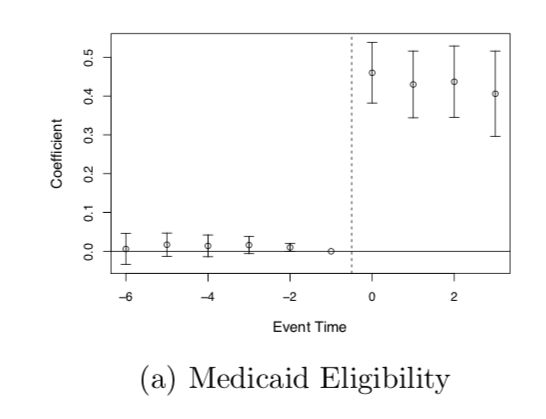
\includegraphics[height=0.60\textheight,keepaspectratio]{figures/Miller_Medicaid1.png}
\end{center}
\vspace{-0.2em}
\begin{center}
\footnotesize\color{warmgray}\itshape
\highlight{Did the policy move people onto Medicaid?} Yes --- enrollment rose sharply in expansion states post-2014, flat in non-expansion states. If the law didn't actually \textit{do} something, nothing downstream is attributable to it.
\end{center}
\end{frame}

\begin{frame}{Bite \#2: any-insurance coverage also rose}
\begin{center}
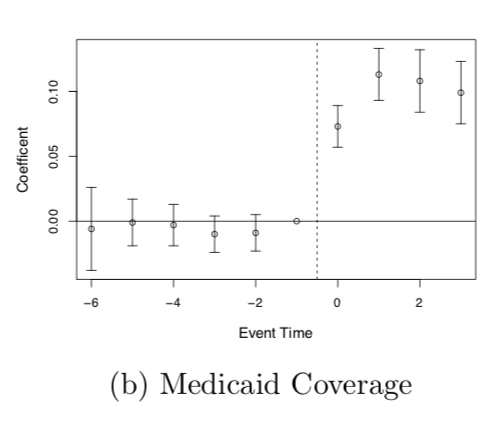
\includegraphics[height=0.60\textheight,keepaspectratio]{figures/Miller_Medicaid2.png}
\end{center}
\vspace{-0.2em}
\begin{center}
\footnotesize\color{warmgray}\itshape
\highlight{Did Medicaid crowd out private insurance, or did total coverage rise?} Coverage rose broadly in expansion states --- take-up is real, not mere substitution from one insurer to another.
\end{center}
\end{frame}

\begin{frame}{Bite \#3: the uninsured rate fell in expansion states}
\begin{center}
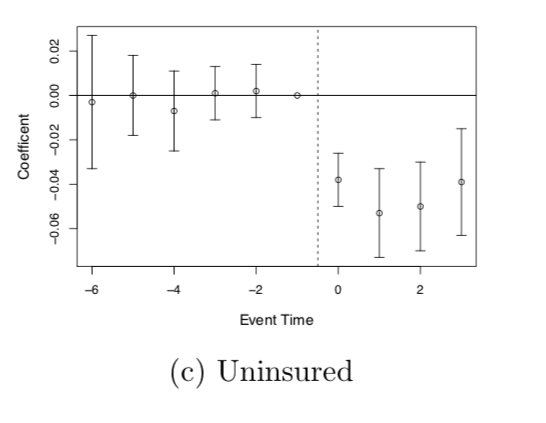
\includegraphics[height=0.60\textheight,keepaspectratio]{figures/Miller_Medicaid3.png}
\end{center}
\vspace{-0.2em}
\begin{center}
\footnotesize\color{warmgray}\itshape
\highlight{Third measure, same story.} Uninsured rate dropped sharply in expansion states post-2014 and stayed flat in non-expansion states. Three independent measures of bite all point the same direction.
\end{center}
\end{frame}

\begin{frame}{Five pieces --- now falsify}
\vspace{0.5em}
\begin{enumerate}\setlength\itemsep{0.7em}
  \item \textcolor{warmgray}{\textit{Bite}} \quad {\color{accent}\checkmark}
  \item \textcolor{warmgray}{\textit{Event study}}
  \item \textbf{Falsification} --- a rival theory fails on a placebo group or outcome.
  \item \textcolor{warmgray}{\textit{Main result}}
  \item \textcolor{warmgray}{\textit{Mechanism}}
\end{enumerate}
\vspace{0.5em}
\meta{A rival explanation: some 2014 shock hit expansion states. If true, it would also hit the 65$+$ population. It didn't.}
\end{frame}

\begin{frame}{Falsification: same model, 65+ population --- no effect}
\begin{center}
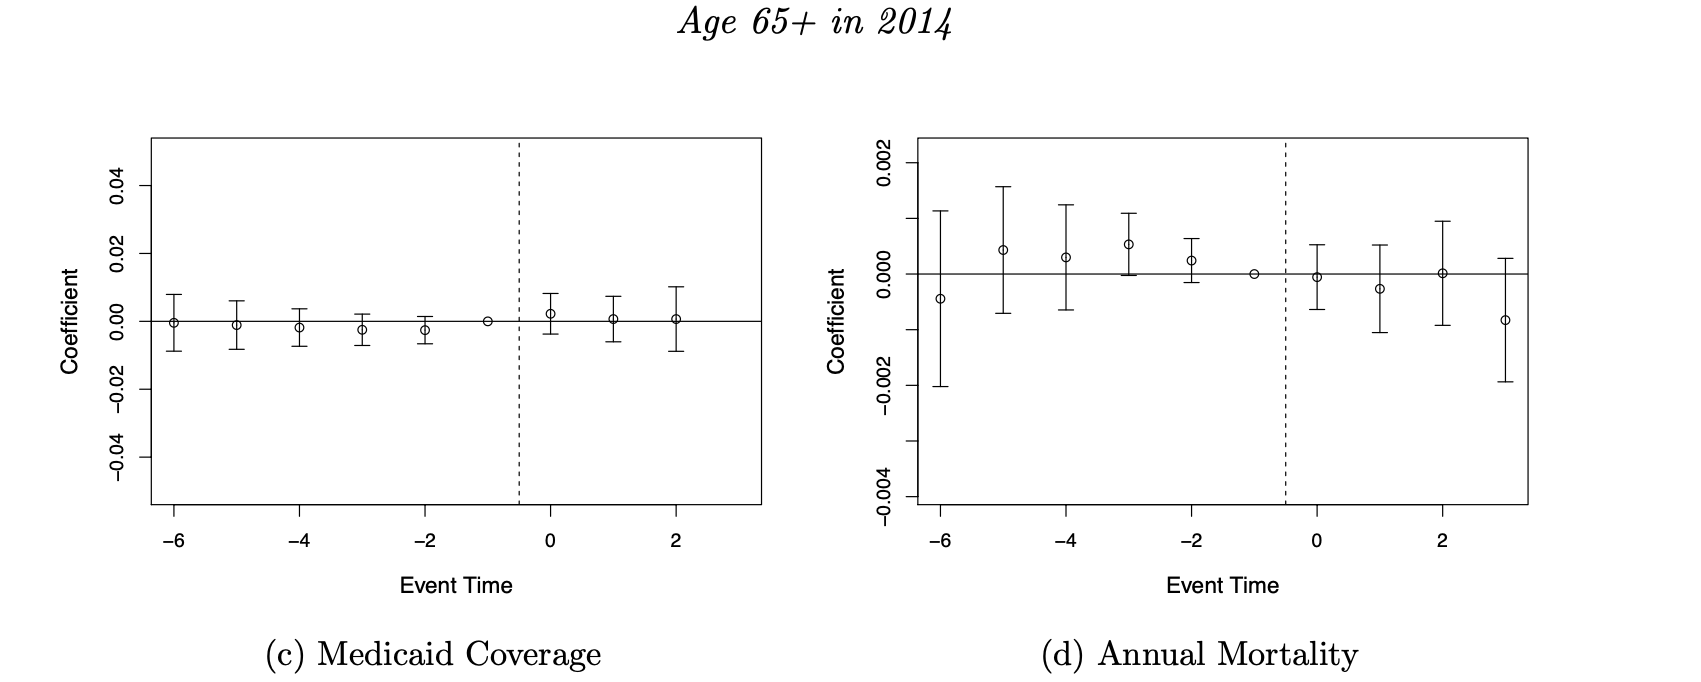
\includegraphics[height=0.60\textheight,keepaspectratio]{figures/placebo_medicaid.png}
\end{center}
\vspace{-0.2em}
\begin{center}
\footnotesize\color{warmgray}\itshape
\highlight{Same states, same years, same model --- but run on the 65$+$ population.} They all have Medicare, so Medicaid expansion shouldn't touch their mortality. A rival story (``some 2014 shock hit expansion states'') would predict a mortality effect here. It didn't appear. \highlight{Rival rejected.}
\end{center}
\end{frame}

\begin{frame}{Five pieces --- event study and main result}
\vspace{0.5em}
\begin{enumerate}\setlength\itemsep{0.7em}
  \item \textcolor{warmgray}{\textit{Bite}} \quad {\color{accent}\checkmark}
  \item \textbf{Event study} --- pre/post dynamics around the treatment date.
  \item \textcolor{warmgray}{\textit{Falsification}} \quad {\color{accent}\checkmark}
  \item \textbf{Main result} --- the DiD on the outcome that matters.
  \item \textcolor{warmgray}{\textit{Mechanism}}
\end{enumerate}
\vspace{0.5em}
\meta{Flat pre-trends build credibility. The post-2014 break is the result.}
\end{frame}

\begin{frame}{Main result: $\approx 9.2\%$ reduction in near-elderly mortality}
\begin{center}
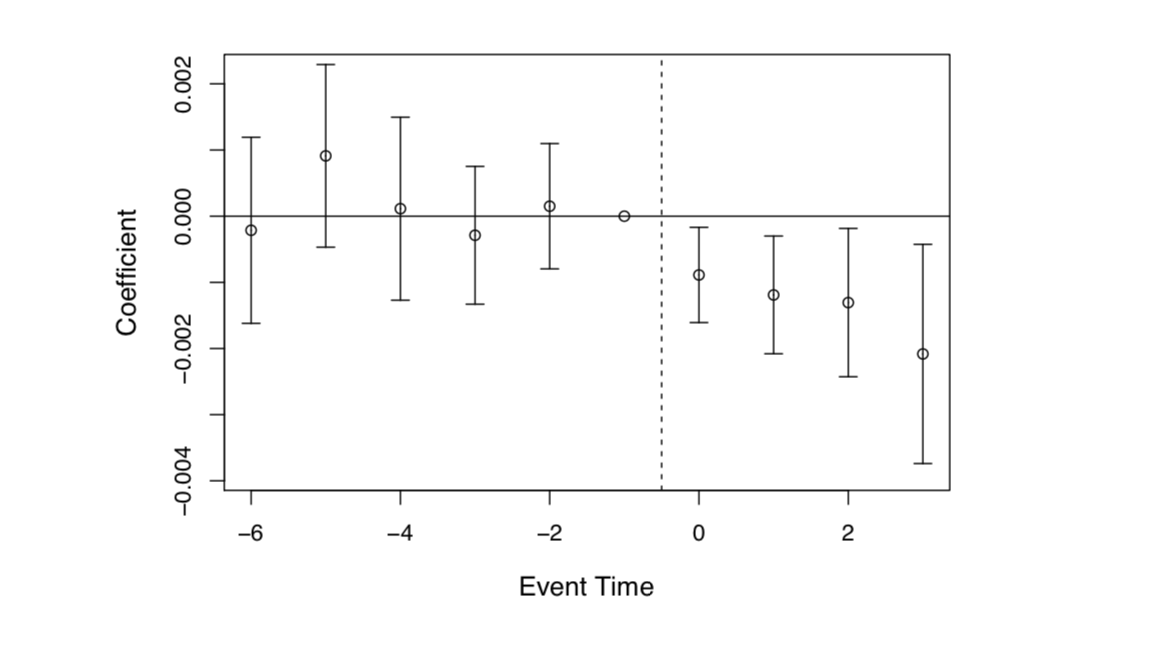
\includegraphics[height=0.50\textheight,keepaspectratio]{figures/Miller_Medicaid4.png}
\end{center}
\vspace{-0.1em}
\footnotesize
\begin{itemize}\setlength\itemsep{2pt}
  \item Post-2014: mortality declines in expansion states. \;\highlight{$\approx 9.2\%$ reduction.}
  \item Pre-period $\hat\beta_k$ near zero. Wide CIs --- but the event study + falsification + bite tell the full story.
  \item A critic must now explain bite \textit{and} falsification \textit{and} the dynamic post-trend simultaneously.
\end{itemize}
\end{frame}

\begin{frame}{Five pieces --- mechanism}
\vspace{0.5em}
\begin{enumerate}\setlength\itemsep{0.7em}
  \item \textcolor{warmgray}{\textit{Bite}} \quad {\color{accent}\checkmark}
  \item \textcolor{warmgray}{\textit{Event study}} \quad {\color{accent}\checkmark}
  \item \textcolor{warmgray}{\textit{Falsification}} \quad {\color{accent}\checkmark}
  \item \textcolor{warmgray}{\textit{Main result}} \quad {\color{accent}\checkmark}
  \item \textbf{Mechanism} --- the causal pathway from $D$ to $Y$.
\end{enumerate}
\vspace{0.5em}
\meta{What \textit{kind} of mortality falls? Disease-specific decomposition tells us where Medicaid is operating.}
\end{frame}

\begin{frame}{Mechanism: disease-related deaths fall}
\vspace{0.3em}
\begin{itemize}\setlength\itemsep{0.5em}
  \item Mechanisms are the part of a result that is \highlight{transportable} to other settings and populations.
  \item Reduced-form results often bundle several mechanisms --- decompositions separate them.
  \item Here: \highlight{disease-related deaths fall} (cardiovascular, respiratory, infectious disease); injury deaths do not.
  \item Consistent with \highlight{chronic-disease management} --- exactly what insurance-mediated access to care would facilitate.
\end{itemize}
\vspace{0.4em}
\emphbox{Mechanisms tell you \textit{why} it worked and \textit{how far the result generalizes}. If the mechanism is access to preventive care, the finding transfers to other populations with similar unmet preventive needs.}
\end{frame}

\begin{frame}{The five pieces, all five present in Medicaid}
\vspace{0.3em}
\begin{center}
\small
\begin{tabular}{@{}lll@{}}
\toprule
\textbf{Piece} & \textbf{Test} & \textbf{Result} \\
\midrule
Bite          & Enrollment, any-insurance, uninsured rate   & \highlight{All three move} \\
Event study   & Pre-$\hat\beta_k$ near zero; 2014 break     & \highlight{Flat pre-trends} \\
Falsification & Same model, 65$+$ population (Medicare)     & \highlight{No effect} \\
Main result   & DiD on near-elderly mortality                & \highlight{$-9.2\%$} \\
Mechanism     & Disease-specific decomposition               & \highlight{Chronic disease} \\
\bottomrule
\end{tabular}
\end{center}
\vspace{0.4em}
\meta{A critic must explain all five simultaneously. The evidentiary burden is now very high.}
\end{frame}

%% ============================================================
%% PART 9. COVARIATES IN DiD
%% (frames from 02-covariates-short.tex)
%% ============================================================
\remixsection{Covariates in DiD}

%%
\begin{frame}{Recall: the 2$\times$2 is DiD --- six equivalent forms}
\vspace{0.2em}
{\footnotesize
\begin{enumerate}\setlength\itemsep{0.25em}

  \item $\underbrace{\bigl[\,\mathbb{E}[Y|D{=}1,t]
         - \mathbb{E}[Y|D{=}1,t{-}1]\,\bigr]}_{\text{first difference}}
        -\;
        \underbrace{\bigl[\,\mathbb{E}[Y|D{=}0,t]
         - \mathbb{E}[Y|D{=}0,t{-}1]\,\bigr]}_{\text{first difference}}$

  \item $\underbrace{\bigl[\,\mathbb{E}[Y|D{=}1,t]
         - \mathbb{E}[Y|D{=}0,t]\,\bigr]}_{\text{group difference}}
        -\;
        \underbrace{\bigl[\,\mathbb{E}[Y|D{=}1,t{-}1]
         - \mathbb{E}[Y|D{=}0,t{-}1]\,\bigr]}_{\text{group difference}}$

  \item $Y = \alpha_1 + \alpha_2\,\mathrm{Post} + \alpha_3\,D
         + \delta\,(\mathrm{Post}\times D) + \varepsilon$
        \hfill{\color{warmgray}\itshape saturated regression}

  \item $Y = \alpha_1 + \tau_t + \sigma_i
         + \delta\,(\mathrm{Post}\times D) + \varepsilon$
        \hfill{\color{warmgray}\itshape two-way fixed effects}

  \item $\Delta Y_i = \alpha_1 + \delta\,D_i + \varepsilon_i$
        \hfill{\color{warmgray}\itshape first-difference / horizontal regression}

  \item $\Delta\bar{Y}_G = \alpha_1 + \delta\,\mathrm{Post}_G + \varepsilon_G$
        \hfill{\color{warmgray}\itshape group / vertical regression}

\end{enumerate}
}
\vspace{0.3em}
\emphbox{All six are \textbf{numerically identical}.}
\end{frame}

\begin{frame}{The 2$\times$2 DiD estimand}
\vspace{0.8em}
\begin{center}
\large
$\underbrace{\widehat{\delta}_{\text{DiD}}}_{\text{what we estimate}}
 \;=\;
 \underbrace{\text{ATT}}_{\text{what we want}}
 \;+\;
 \underbrace{\bigl[\,\mathbb{E}[\Delta Y(0)\mid D{=}1]
              - \mathbb{E}[\Delta Y(0)\mid D{=}0]\,\bigr]}_{\text{PT bias}}$
\end{center}
\vspace{0.8em}
\begin{center}\color{warmgray}\small
Treatment $=$ college education. \quad Outcome $=$ wages.\\
Parallel trends requires the PT bias term to equal zero.
\end{center}
\end{frame}

%%
\begin{frame}{A thought experiment}
\vspace{0.5em}
\begin{center}
\begin{tabular}{@{}ll@{}}
\toprule
\textbf{Group} & \textbf{Untreated wage trend $\Delta Y(0)$} \\
\midrule
Male workers   & $+10$ per year \\
Female workers & $+8$\phantom{0} per year \\
\bottomrule
\end{tabular}
\end{center}
\vspace{0.8em}
\begin{center}
\textbf{Case 1:} $D{=}1$ is 75\% male. \quad $D{=}0$ is 75\% male.\\[0.4em]
\color{warmgray}\small Will parallel trends hold?
\end{center}
\end{frame}

%%
\begin{frame}{Case 1: show the work}
\vspace{0.6em}
\begin{center}
\begin{tabular}{@{}lll@{}}
\toprule
& \textbf{Calculation} & \textbf{Result} \\
\midrule
$\mathbb{E}[\Delta Y(0)\mid D{=}1]$ & $0.75\times10 + 0.25\times8$ & $9.5$ \\[0.3em]
$\mathbb{E}[\Delta Y(0)\mid D{=}0]$ & $0.75\times10 + 0.25\times8$ & $9.5$ \\
\bottomrule
\end{tabular}
\end{center}
\vspace{0.8em}
\begin{center}
Parallel trends holds? \quad \textcolor{forest}{\textbf{Yes.}}\\[0.3em]
\color{warmgray}\small $\widehat{\delta}_{\text{DiD}} = \text{ATT}$ \;\checkmark
\end{center}
\end{frame}

%%
\begin{frame}{Case 2: unequal composition}
\vspace{0.5em}
\begin{center}
\begin{tabular}{@{}ll@{}}
\toprule
& \textbf{\% male} \\
\midrule
$D{=}1$ (college educated) & 75\% \\
$D{=}0$ (no college)       & 25\% \\
\bottomrule
\end{tabular}
\end{center}
\vspace{0.8em}
\begin{center}
\color{warmgray}\small
Same wage trends as before ($+10$ male, $+8$ female).\\
Will parallel trends hold now?
\end{center}
\end{frame}

%%
\begin{frame}{Case 2: show the work}
\vspace{0.6em}
\begin{center}
\begin{tabular}{@{}lll@{}}
\toprule
& \textbf{Calculation} & \textbf{Result} \\
\midrule
$\mathbb{E}[\Delta Y(0)\mid D{=}1]$ & $0.75\times10 + 0.25\times8$ & $9.5$ \\[0.3em]
$\mathbb{E}[\Delta Y(0)\mid D{=}0]$ & $0.25\times10 + 0.75\times8$ & $8.5$ \\
\bottomrule
\end{tabular}
\end{center}
\vspace{0.8em}
\begin{center}
Parallel trends holds? \quad \textcolor{red}{\textbf{No.}}\\[0.3em]
\color{warmgray}\small
$\widehat{\delta}_{\text{DiD}} \;\neq\; \text{ATT}$
\quad because PT bias $= 9.5 - 8.5 = 1.0 \neq 0$
\end{center}
\end{frame}

%%
\begin{frame}{Why? Imbalance on a trend-causing covariate}
\vspace{0.8em}
\begin{center}
DiD does \textbf{not} require the two groups to look the same on \emph{levels}.\\[0.6em]
DiD \textbf{does} require the same $Y(0)$ \emph{trends}.\\[0.8em]
\end{center}
\emphbox{Imbalance in a covariate that \emph{causes} $Y(0)$ trends\\
will \textbf{mechanically} break parallel trends.}
\end{frame}

%%
\begin{frame}{Fix: control for sex}
\vspace{0.6em}
\begin{center}
If sex is the only covariate driving differential trends,\\
then \emph{conditioning on sex} removes the PT bias.
\end{center}
\vspace{0.6em}
\begin{center}
Several ways to do this:
\end{center}
\vspace{0.3em}
\begin{enumerate}\setlength\itemsep{0.4em}
  \item TWFE saturated regressions
  \item Inverse probability weighting (IPW)
  \item Outcome regression (OR)
  \item Doubly robust (DR)
\end{enumerate}
\vspace{0.5em}
\begin{center}\color{warmgray}\small
We will discuss all four.
\end{center}
\end{frame}

%%
\begin{frame}{For conditioning to work: conditional PT}
\vspace{0.6em}
\begin{center}
We need parallel trends \emph{within} each group:
\end{center}
\vspace{0.4em}
\begin{enumerate}\setlength\itemsep{0.5em}
  \item Male treated workers have the \emph{same} $Y(0)$ trend as male control workers
  \item Female treated workers have the \emph{same} $Y(0)$ trend as female control workers
\end{enumerate}
\vspace{0.6em}
\emphbox{Conditional PTA: \;\;
$\mathbb{E}[\Delta Y(0)\mid D{=}1,\,X] = \mathbb{E}[\Delta Y(0)\mid D{=}0,\,X]$
\quad for all $X$}
\end{frame}

%% ====================================================================
%% PART 1 — OLS SPECIFICATIONS
%% ====================================================================

\begin{frame}{The standard TWFE with additive $X$}
\vspace{0.6em}
\begin{center}
\large
$Y_{it} \;=\; \alpha_i + \lambda_t
      + \delta\,(D_i \times \mathrm{Post}_t)
      + \boldsymbol{\beta}\,X_i
      + \varepsilon_{it}$
\end{center}
\vspace{0.5em}
\begin{center}
Two hidden assumptions:
\begin{enumerate}
  \item Returns to $X$ are \textbf{constant over time}
  \item Treatment effect is \textbf{the same for all $X$}
\end{enumerate}
\end{center}
\vspace{0.4em}
\emphbox{\textbf{Fatal problem:} if $X_i$ is time-invariant, it is collinear with $\alpha_i$
and drops out --- whether you use unit fixed effects \emph{or} a saturated dummy
specification. An additive, separable $X$ cannot deliver conditional parallel
trends if the covariate is absorbed before it can do any work.}
\end{frame}

%% ----------
%%
\begin{frame}{What if returns to $X$ change over time?}
\vspace{0.3em}
\begin{center}\color{warmgray}\small
Example: discrimination against women is not constant --- $\beta_{\text{post}} \neq \beta_{\text{pre}}$.
\end{center}
\vspace{0.4em}

Allow time-varying returns in the DGP:
\[
Y_{it}(0) = \alpha_i + \gamma_t + \beta_t\, X_i
\]

Write out the \textbf{post} and \textbf{pre} equations for unit $i$:

\begin{align*}
Y_{i,\text{post}}(0) &= \alpha_i + \gamma_{\text{post}} + \beta_{\text{post}}\, X_i \\[4pt]
Y_{i,\text{pre}}(0)  &= \alpha_i + \gamma_{\text{pre}}  + \beta_{\text{pre}}\,  X_i
\end{align*}

Subtract (post $-$ pre):
\[
\Delta Y_i(0)
  = \underbrace{(\gamma_{\text{post}} - \gamma_{\text{pre}})}_{\Delta\gamma}
  + \underbrace{(\beta_{\text{post}}  - \beta_{\text{pre}})}_{\Delta\beta}
    \cdot X_i
\]
\end{frame}

%%
\begin{frame}{Now take expectations by group}
\vspace{0.4em}

Starting from $\;\Delta Y_i(0) = \Delta\gamma + \Delta\beta\cdot X_i$, condition on treatment status:

\begin{align*}
E[\Delta Y(0)\mid D{=}1] &= \Delta\gamma + \Delta\beta\cdot E[X\mid D{=}1] \\[4pt]
E[\Delta Y(0)\mid D{=}0] &= \Delta\gamma + \Delta\beta\cdot E[X\mid D{=}0]
\end{align*}

\vspace{0.3em}
Parallel trends bias:
\[
\underbrace{E[\Delta Y(0)\mid D{=}1] - E[\Delta Y(0)\mid D{=}0]}_{\text{PT bias}}
  \;=\;
  \Delta\beta\;\cdot\;
  \bigl(\,E[X\mid D{=}1] - E[X\mid D{=}0]\,\bigr)
\]

\vspace{0.4em}
\emphbox{PT fails whenever \textbf{both}: returns shift ($\Delta\beta \neq 0$) \textbf{and} groups are imbalanced on $X$.}
\end{frame}

%%
\begin{frame}[fragile]{Fix for Bias \#1: interact $\mathrm{Post} \times X$}
\vspace{0.4em}
\begin{center}
$Y_{it} \;=\; \alpha_i + \lambda_t
      + \delta\,(D_i \times \mathrm{Post}_t)
      + \boldsymbol{\beta}\,X_i
      + {\color{accent}\boldsymbol{\gamma}\,(\mathrm{Post}_t \times X_i)}
      + \varepsilon_{it}$
\end{center}
\vspace{0.3em}
\begin{center}\color{warmgray}\small
$\boldsymbol{\gamma}$ absorbs any shift in returns to $X$ between pre and post (Spec B in the lab).
\end{center}
\vspace{0.3em}
\begin{lstlisting}[language={[ANSI]C},basicstyle=\ttfamily\scriptsize]
reg re i.post##i.ever_treated ///
    i.post##c.age i.post##c.agesq i.post##c.agecube ///
    i.post##c.educ i.post##c.educsq ///
    i.post##i.marr i.post##i.nodegree i.post##i.black i.post##i.hisp ///
    i.post##c.re74 i.post##i.u74, robust
\end{lstlisting}
\end{frame}

%% ====================================================================
%% BIAS #2 — HETEROGENEOUS TREATMENT EFFECTS
%% ====================================================================
\remixsection{Bias \#2: Heterogeneous Treatment Effects}

%%
\begin{frame}{What if the effect of college differs by sex?}
\vspace{0.5em}
\begin{center}
Previously we worried about \textbf{trends in $Y(0)$} being unequal across groups.\\[0.5em]
Now the concern is different:
\[
\mathbb{E}[Y(1) - Y(0)\mid \text{Male}] \;\neq\; \mathbb{E}[Y(1) - Y(0)\mid \text{Female}]
\]
\end{center}
\vspace{0.4em}
\begin{center}\color{warmgray}\small
Do the rich and the poor get the same return to college?\\
Do workers in cities and towns get the same return?\\[0.4em]
If not, \textbf{and} the treatment group is imbalanced on these covariates,\\
the 2$\times$2 DiD will not recover the ATT.
\end{center}
\end{frame}

%%
\begin{frame}{Proof, step 1 --- the TWFE model and conditional PT}
\vspace{0.3em}
\textbf{The TWFE model with one covariate $X$:}
\[
Y_{it} \;=\; \alpha_i + \gamma_t + \delta\,(T_t \times D_i) + \beta\, X_i + \varepsilon_{it}
\]
\textbf{Conditional parallel trends} says, for each value of $X$:
\[
\mathbb{E}[Y(0)_{\text{post}} - Y(0)_{\text{pre}} \mid D{=}1,\, X]
\;=\;
\mathbb{E}[Y(0)_{\text{post}} - Y(0)_{\text{pre}} \mid D{=}0,\, X]
\]
Rearranged --- the missing counterfactual for the treated is identified:
\[
\mathbb{E}[Y(0)_{\text{post}} \mid D{=}1, X]
\;=\;
\mathbb{E}[Y_{\text{pre}} \mid D{=}1, X]
+ \mathbb{E}[Y_{\text{post}} \mid D{=}0, X]
- \mathbb{E}[Y_{\text{pre}} \mid D{=}0, X]
\]
\end{frame}

%%
\begin{frame}{Proof, step 2 --- plug TWFE in: the slopes look the same}
\vspace{0.3em}
\textbf{From the TWFE model, observed conditional means:}
\begin{align*}
\mathbb{E}[Y_{\text{pre}}  \mid D{=}1, X] &= \alpha_1 + \alpha_3 + \beta\, X \\[3pt]
\mathbb{E}[Y_{\text{post}} \mid D{=}0, X] &= \alpha_1 + \alpha_2 + \beta\, X \\[3pt]
\mathbb{E}[Y_{\text{pre}}  \mid D{=}0, X] &= \alpha_1 + \beta\, X
\end{align*}
\textbf{Counterfactual for treated (step 1 identity):}
\[
\mathbb{E}[Y(0)_{\text{post}} \mid D{=}1, X] \;=\; \alpha_1 + \alpha_2 + \alpha_3 + \beta\, X
\]
\textbf{Treated outcome, post:} $\;\mathbb{E}[Y(1)_{\text{post}} \mid D{=}1, X] = \alpha_1 + \alpha_2 + \alpha_3 + \delta + \beta\, X$\\[0.4em]
\begin{center}\color{warmgray}\small
Both potential outcomes carry the \textit{same} $\beta$. Subtract: ATT $= \delta$. \textit{Suspiciously clean.}
\end{center}
\end{frame}

%%
\begin{frame}{Proof, step 3 --- what if $Y(1)$ and $Y(0)$ have different slopes in $X$?}
\vspace{0.3em}
\textbf{Let the slopes differ:} write $\beta_1$ for the $Y(1)$ slope, $\beta_2$ for $Y(0)$:
\begin{align*}
\mathbb{E}[Y(1)_{\text{post}} \mid D{=}1, X] &= \alpha_1 + \alpha_2 + \alpha_3 + \delta + \beta_1\, X \\[3pt]
\mathbb{E}[Y(0)_{\text{post}} \mid D{=}1, X] &= \alpha_1 + \alpha_2 + \alpha_3 \phantom{\;+\;\delta} + \beta_2\, X
\end{align*}
\textbf{True ATT given $X$:}
\[
\text{ATT}(X) \;=\; \delta + (\beta_1 - \beta_2)\, X
\]
\begin{itemize}\setlength\itemsep{0.3em}\small
  \item If $\beta_1 \neq \beta_2$, the treatment effect \textit{depends on} $X$
  \item TWFE fits one $\beta$, not two --- so $\hat\delta$ recovers ATT only if $\beta_1 = \beta_2$
\end{itemize}
\end{frame}

%%
\begin{frame}{Proof, step 4 --- TWFE imposes homogeneous $\delta$ in $X$}
\vspace{0.3em}
\emphbox{\textbf{Assumption:} TWFE-with-$X$ requires the treatment effect to be the same
at every value of $X$.}
\vspace{0.5em}
\begin{itemize}\setlength\itemsep{0.5em}
  \item If $X$ is \textbf{sex}: effect must be equal for men and women
  \item If $X$ is \textbf{income}: effect must be equal at \$1 and at \$1{,}000{,}000
  \item If $X$ is \textbf{age}: effect must be equal at 25 and at 65
\end{itemize}
\vspace{0.5em}
\begin{center}\color{warmgray}\small
OLS doesn't warn you that you're making this assumption. The math does.\\
If effects actually vary with $X$, TWFE averages across the variation\\
and returns a weighted parameter you didn't ask for.
\end{center}
\end{frame}

%%
\begin{frame}[fragile]{Fix for Bias \#2: saturate treatment with $X$}
\vspace{0.2em}
\begin{enumerate}\setlength\itemsep{0.4em}\small
  \item \textbf{Run a saturated regression on first differences} --- interact treatment with every $X$
  \item \textbf{Predict $\Delta Y(1)$ and $\Delta Y(0)$ for each unit} --- average the gap in the treated group
\end{enumerate}
\vspace{0.3em}
\begin{lstlisting}[language={[ANSI]C},basicstyle=\ttfamily\tiny]
* 1. Saturated regression on first differences
reg dy i.ever_treated ///
    i.ever_treated#c.age i.ever_treated#c.agesq ///
    i.ever_treated#c.educ i.ever_treated#c.educsq ///
    i.ever_treated#i.marr i.ever_treated#i.nodegree ///
    i.ever_treated#i.black i.ever_treated#i.hisp ///
    i.ever_treated#c.re74 i.ever_treated#i.u74 ///
    $X, robust

* 2. Predict potential outcomes; average the gap in the treated group
replace ever_treated = 1
quietly predict dy_hat_1, xb
replace ever_treated = 0
quietly predict dy_hat_0, xb
replace ever_treated = evt_orig          // restore
gen tau_sat = dy_hat_1 - dy_hat_0
quietly sum tau_sat if ever_treated == 1 // ATT = r(mean)
\end{lstlisting}
\end{frame}

%% ====================================================================
%% BIAS #3 — TIME-INVARIANT COVARIATES
%% ====================================================================

%%
\begin{frame}{Bias \#3: time-invariant covariates get absorbed}
\vspace{0.6em}
\begin{center}
If you need $X_i$ for conditional PT, but $X_i$ doesn't change over time,\\
TWFE will \textbf{delete it}.
\end{center}
\vspace{0.5em}
\begin{center}\color{warmgray}\small
TWFE ``demeans'' the data. The mean of a constant is itself.\\
So $X_i - \bar{X}_i \equiv 0$ --- it drops out of the regression entirely.
\end{center}
\vspace{0.5em}
\emphbox{\textbf{Fix:} include $X_i \times \mathrm{Post}_t$ instead. \;The Post interaction is time-varying,\\
so it survives demeaning and can do the work of conditioning on $X$.}
\end{frame}

%% ====================================================================
%% SUMMARY
%% ====================================================================

%%
\begin{frame}{Three biases --- one family of fixes}
\vspace{0.3em}
{\small
\begin{tabular}{@{}lll@{}}
\toprule
\textbf{Bias} & \textbf{What TWFE imposes} & \textbf{Fix} \\
\midrule
\#1 Trend imbalance
  & $\beta$ constant pre and post
  & $\mathrm{Post}\times X$ \\[4pt]
\#2 Heterogeneous TE
  & $\delta$ same at every $X$
  & $D\times X$ (saturate treatment) \\[4pt]
\#3 Time-invariant $X$
  & $X_i$ survives demeaning
  & $\mathrm{Post}\times X$ (same fix as \#1) \\
\bottomrule
\end{tabular}
}
\vspace{0.5em}
\emphbox{Most researchers include additive $X$ and call it a day. That is the wrong spec.
To fix all three you need both $\mathrm{Post}\times X$ and $D\times X$.
It is rare to see this in published work.}
\end{frame}

%%
\begin{frame}{Now: the LaLonde application}
\vspace{1.2em}
\begin{center}
\Large
Switch to \textbf{02b-lalonde.pdf}\\[0.8em]
\color{warmgray}\normalsize
We will walk through the code together,\\
then return here for OR, IPW, and DR.
\end{center}
\end{frame}

%% ====================================================================
%% ALTERNATIVE ESTIMATORS
%% ====================================================================
\remixsection{Alternative Estimators}

%%
\begin{frame}{Three more estimators}
\vspace{0.8em}
\begin{center}
Now we will look at three more estimators.\\[0.5em]
These are alternatives to the regression-based specs we just covered.
\end{center}
\vspace{0.6em}
\begin{enumerate}\setlength\itemsep{0.5em}
  \item \highlight{IPW} --- reweight controls to look like treated
  \item \highlight{Outcome regression (OR)} --- model the control trend, impute the counterfactual
  \item \highlight{Doubly robust (DR)} --- combine both; consistent if \textit{either} is right
\end{enumerate}
\end{frame}

\begin{frame}{IPW: reweight the controls to look like the treated}
\vspace{1.0em}
\begin{center}
\large
$\widehat{\mathrm{ATT}}_{\mathrm{IPW}}
  \;=\; \dfrac{1}{\bar{D}}\,\dfrac{1}{n}
        \displaystyle\sum_{i=1}^{n}
        \frac{D_i - \hat{p}(X_i)}{1 - \hat{p}(X_i)}
        \;\Delta Y_i$
\end{center}
\vspace{0.8em}
\begin{center}
\color{warmgray}\small
$\hat{p}(X_i) = \widehat{\Pr}(D_i=1\mid X_i)$ \quad (propensity score)
\qquad
$\Delta Y_i = Y_{i,\mathrm{post}} - Y_{i,\mathrm{pre}}$
\end{center}
\end{frame}

%% ----------
\begin{frame}{IPW: five steps}
\vspace{0.8em}
\begin{enumerate}\setlength\itemsep{0.5em}
  \item \highlight{Estimate $\hat{p}(X)$.} \;Logit of $D_i$ on $X_i$.
  \item \highlight{Check overlap.} \;Plot $\hat{p}$ by treatment status. Trim if needed.
  \item \highlight{Construct weights.} \;$w_i = (D_i - \hat{p}(X_i)) / (1 - \hat{p}(X_i))$.
  \item \highlight{Weighted average.} \;$\widehat{\mathrm{ATT}} = \sum w_i\,\Delta Y_i \;/\; n_T$.
  \item \highlight{Standard error.} \;Bootstrap or influence function.
\end{enumerate}
\end{frame}

%% ----------
\begin{frame}{Overlap is non-negotiable}
\vspace{1.2em}
\begin{center}
\large
If $\hat{p}(X_i) \to 1$ for a control unit, its weight $\to \infty$.\\[0.8em]
\highlight{No overlap = no valid counterfactual.}\\[0.8em]
\color{warmgray}\normalsize
This is a data problem. No estimator fixes it.
\end{center}
\end{frame}

%% ====================================================================
%% PART 3 — OR
%% ====================================================================

\begin{frame}{OR --- or ``regression adjustment''}
\vspace{0.6em}
\begin{center}
\large
$\widehat{\mathrm{ATT}}_{\mathrm{OR}}
  \;=\; \dfrac{1}{n_T}
        \displaystyle\sum_{D_i=1}
        \Bigl[\Delta Y_i \;-\; \hat\mu_0(X_i)\Bigr]$
\end{center}
\vspace{0.6em}
\begin{center}
\color{warmgray}\small
$\hat\mu_0(X_i) = \widehat{E}[\Delta Y \mid D{=}0,\,X]$ \quad estimated on controls only
\end{center}
\vspace{0.5em}
\begin{center}
\small
The estimator is increasingly called \textbf{regression adjustment} (RA)\\
in the modern applied literature. Same idea, newer name.
\end{center}
\end{frame}

%% ----------
\begin{frame}{OR: five steps}
\vspace{0.8em}
\begin{enumerate}\setlength\itemsep{0.5em}
  \item \highlight{First-difference.} \;$\Delta Y_i = Y_{i,\mathrm{post}} - Y_{i,\mathrm{pre}}$.
  \item \highlight{Fit outcome model.} \;Regress $\Delta Y$ on $X$ \textit{using controls only}.
  \item \highlight{Predict counterfactual.} \;Evaluate $\hat\mu_0(X_i)$ for each treated unit.
  \item \highlight{Mean gap.} \;ATT $= \overline{\Delta Y}^T - \overline{\hat\mu_0(X)}^T$.
  \item \highlight{Standard error.} \;Bootstrap.
\end{enumerate}
\end{frame}

%%
\begin{frame}{Surprise --- you already know OR}
\vspace{0.8em}
\begin{center}
\large
OR step 2: \emph{``Regress $\Delta Y$ on $X$ using controls only.''}\\[0.8em]
\color{warmgray}\normalsize
That is exactly what the saturated TWFE does.\\[0.4em]
Let's prove it slowly.
\end{center}
\end{frame}

%%
\begin{frame}{Proof, step 1 --- the saturated model}
\vspace{0.4em}
\begin{center}\color{warmgray}\small
Spec C runs this regression on first differences:\end{center}
\vspace{0.3em}
\[
\Delta Y_i \;=\; \underbrace{\alpha}_{\text{intercept}}
            \;+\; \underbrace{\delta\, D_i}_{\text{treatment}}
            \;+\; \underbrace{\beta'\, X_i}_{\text{covariates}}
            \;+\; \underbrace{\tau'\,(D_i \times X_i)}_{\text{treatment interactions}}
            \;+\; \varepsilon_i
\]
\vspace{0.4em}
\begin{center}
$D_i \in \{0, 1\}$ \quad and \quad \textbf{every} element of $X_i$ is interacted with $D_i$.
\end{center}
\end{frame}

%%
\begin{frame}{Proof, step 2 --- separate by group}
\vspace{0.3em}
\begin{center}\color{warmgray}\small Plug $D_i = 0$ and $D_i = 1$ into the model:\end{center}
\vspace{0.4em}
\begin{align*}
D_i = 0: \quad \Delta Y_i &= \alpha + \beta'\, X_i + \varepsilon_i \\[6pt]
D_i = 1: \quad \Delta Y_i &= (\alpha + \delta) + (\beta + \tau)'\, X_i + \varepsilon_i
\end{align*}
\vspace{0.4em}
\begin{center}
The two groups have \textbf{entirely different} parameters.\\[0.4em]
\color{warmgray}\small
Controls contribute to $(\alpha,\,\beta)$.\quad
Treated contribute to $(\alpha+\delta,\,\beta+\tau)$.
\end{center}
\end{frame}

%%
\begin{frame}{Proof, step 3 --- OLS separates completely}
\vspace{0.4em}
\begin{center}\color{warmgray}\small
Re-label: \;$a_0 = \alpha$, \;$b_0 = \beta$, \;$a_1 = \alpha+\delta$, \;$b_1 = \beta+\tau$.
\end{center}
\vspace{0.3em}
The OLS objective is:
\[
\min_{a_0,b_0,a_1,b_1}
  \underbrace{\sum_{D_i=0}\!\bigl(\Delta Y_i - a_0 - b_0'\,X_i\bigr)^{\!2}}_{\text{only controls}}
  \;+\;
  \underbrace{\sum_{D_i=1}\!\bigl(\Delta Y_i - a_1 - b_1'\,X_i\bigr)^{\!2}}_{\text{only treated}}
\]
\vspace{0.3em}
\begin{center}
The two sums share \textbf{no parameters}.\\[0.4em]
\emphbox{$(\hat a_0,\,\hat b_0)$ \;=\; OLS of $\Delta Y$ on $X$ \textbf{using controls only.}}
\end{center}
\end{frame}

%%
\begin{frame}{Proof, step 4 --- Spec C and OR make the same imputation}
\vspace{0.4em}
\begin{center}\color{warmgray}\small
For a treated unit $i$, what does each estimator predict as $\Delta Y_i(0)$?
\end{center}
\vspace{0.5em}
\begin{center}
\begin{tabular}{@{}ll@{}}
\toprule
\textbf{Spec C (saturated TWFE)} & set $D_i{=}0$: \quad $\hat a_0 + \hat b_0'\,X_i$ \\[6pt]
\textbf{OR / regression adjustment} & control OLS: \quad $\hat a_0 + \hat b_0'\,X_i$ \\
\bottomrule
\end{tabular}
\end{center}
\vspace{0.6em}
\emphbox{Identical prediction $\;\Rightarrow\;$ identical ATT.\quad
\textbf{Spec C is OR.}}
\end{frame}

%%
\begin{frame}{One estimator, two names --- just like the 2$\times$2}
\vspace{0.6em}
\begin{center}
Recall: six formulas for the 2$\times$2, all giving the same number.\\[0.6em]
Same principle here.\\[0.8em]
\end{center}
\emphbox{Saturated TWFE (Spec C) and outcome regression (OR / RA)\\
are \textbf{the same estimator} expressed two different ways.\\[0.3em]
We will confirm this in the do file: both print \$1{,}770.}
\end{frame}

%% ====================================================================
%% PART 4 — DR
%% ====================================================================

\begin{frame}{DR: two chances to be right}
\vspace{0.8em}
\begin{center}
\large
$\widehat{\mathrm{ATT}}_{\mathrm{DR}}
  \;=\; \dfrac{1}{\bar{D}}\,\dfrac{1}{n}
        \displaystyle\sum_{i=1}^{n}
        \underbrace{\frac{D_i - \hat{p}(X_i)}{1 - \hat{p}(X_i)}}_{\text{IPW correction}}
        \;\cdot\;
        \underbrace{\bigl[\Delta Y_i - \hat\mu_0(X_i)\bigr]}_{\text{OR residual}}$
\end{center}
\end{frame}

%% ----------
\begin{frame}{DR is consistent if \textit{either} model is right --- not both}
\vspace{0.8em}
\begin{center}
\begin{tabular}{lll}
  \toprule
  $\hat\mu_0$ correct & $\hat{p}$ correct & Consistent? \\
  \midrule
  \checkmark & \checkmark & \checkmark \\
  \checkmark & $\times$   & \checkmark \\
  $\times$   & \checkmark & \checkmark \\
  \rowcolor{remixgreenlight}
  $\times$   & $\times$   & \textbf{No} \\
  \bottomrule
\end{tabular}
\end{center}
\vspace{0.5em}
\begin{center}
\color{warmgray}\small
``Doubly robust'' $\neq$ doubly unbeatable.
\end{center}
\end{frame}

%% ====================================================================
%% PART 5 — LAB
%% ====================================================================

\begin{frame}{Lab: ten estimators, one benchmark}
\vspace{0.6em}
\begin{center}
\texttt{Labs/Lalonde-Covariates/lalonde\_all\_specs.do}
\end{center}
\vspace{0.6em}
\begin{center}
\color{warmgray}\small
NSW treated $+$ CPS controls \textperiodcentered\
Pre = 1975, Post = 1978\\[0.4em]
RCT benchmark: \highlight{\$1,794}
\end{center}
\vspace{0.4em}
\begin{center}
Spec 0 (Naive) \textperiodcentered\ Spec A (Additive $X$) \textperiodcentered\ Spec B (Post$\times X$) \textperiodcentered\ Spec C (Saturated)\\[0.3em]
OR by hand \textperiodcentered\ OR \texttt{drdid} \textperiodcentered\
IPW by hand \textperiodcentered\ IPW \texttt{drdid} \textperiodcentered\
DR by hand \textperiodcentered\ DR \texttt{drdid}
\end{center}
\end{frame}

%% ====================================================================
%% PART 6 — MONTE CARLO
%% ====================================================================

\begin{frame}{A Monte Carlo to rank the estimators}
\vspace{0.6em}
\begin{center}
\begin{tabular}{ll}
  Estimators: & TWFE, OR, IPW, DR \\[0.4em]
  DGPs:       & 4 (vary whether OR model and pscore are correct) \\[0.4em]
  $n$:        & 1{,}000 \quad Replications: 10{,}000 \\[0.4em]
  Report:     & Bias, RMSE, SE, coverage, CI length \\
\end{tabular}
\end{center}
\vspace{0.5em}
\begin{center}
\color{warmgray}\small
When does DR pay off? When does it break?
\end{center}
\end{frame}

%% ----------
\begin{frame}{DGP 1: both models correct}
\vspace{0.4em}
\begin{center}
\small\renewcommand{\arraystretch}{1.3}
\begin{tabular}{@{}lrrrrr@{}}
\toprule
      & \textbf{Bias} & \textbf{RMSE} & \textbf{SE} & \textbf{Coverage} & \textbf{CI length} \\
\midrule
TWFE  & $-20.95$ & $21.12$ & $2.53$ & $0.000$ & $9.91$  \\
OR    & $-0.001$ & $0.10$  & $0.10$ & $0.950$ & $0.40$  \\
IPW   & $+0.026$ & $2.77$  & $2.66$ & $0.952$ & $10.44$ \\
\rowcolor{remixgreenlight}
DR    & $-0.001$ & $0.11$  & $0.11$ & $0.947$ & $0.41$  \\
\bottomrule
\end{tabular}
\end{center}
\vspace{0.3em}
\begin{center}\small\color{warmgray}\itshape
TWFE: coverage zero. \;OR and DR: tight on truth. \;IPW: unbiased but wide.
\end{center}
\end{frame}

%% ----------
\begin{frame}{DGP 1: the sampling distribution}
\vspace{0.3em}
\begin{center}
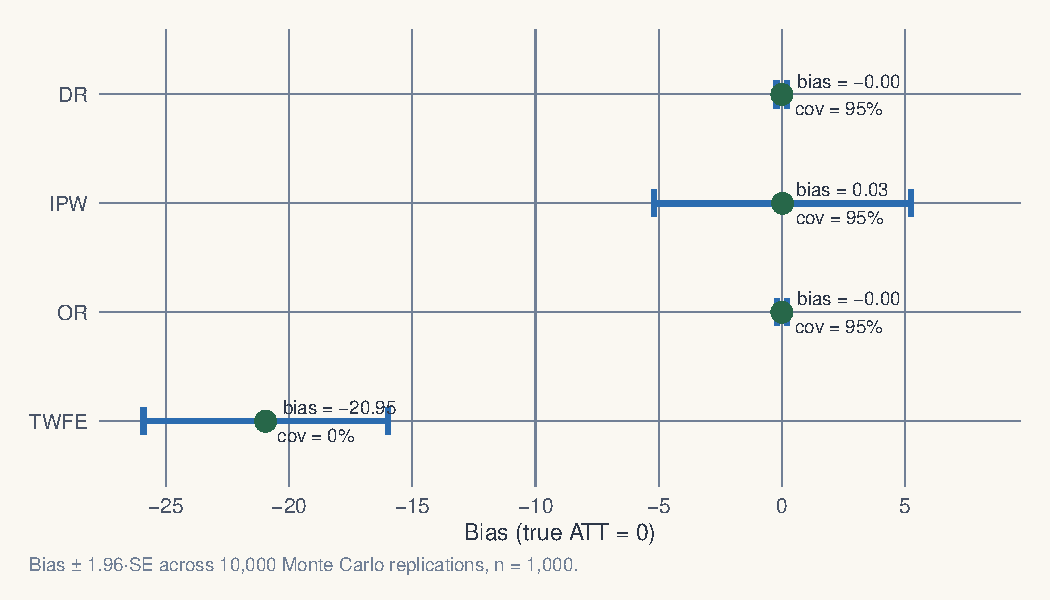
\includegraphics[width=0.68\textwidth]{figures/mc_dr_1.pdf}
\end{center}
\end{frame}

%% ----------
\begin{frame}{DGP 4: both models wrong}
\vspace{0.4em}
\begin{center}
\small\renewcommand{\arraystretch}{1.3}
\begin{tabular}{@{}lrrrrr@{}}
\toprule
      & \textbf{Bias} & \textbf{RMSE} & \textbf{SE} & \textbf{Coverage} & \textbf{CI length} \\
\midrule
TWFE  & $-16.38$ & $16.54$ & $3.63$ & $0.000$ & $14.22$ \\
OR    & $-5.20$  & $5.36$  & $1.29$ & $0.015$ & $5.05$  \\
\rowcolor{remixgreenlight}
IPW   & $-1.08$  & $2.66$  & $2.37$ & $0.949$ & $9.31$  \\
DR    & $-3.19$  & $3.45$  & $1.29$ & $0.308$ & $5.07$  \\
\bottomrule
\end{tabular}
\end{center}
\vspace{0.3em}
\begin{center}\small\color{warmgray}\itshape
DR undercovers at 0.31. IPW wins. Doubly robust $\neq$ doubly unbeatable.
\end{center}
\end{frame}

%% ----------
\begin{frame}{DGP 4: the sampling distribution}
\vspace{0.3em}
\begin{center}
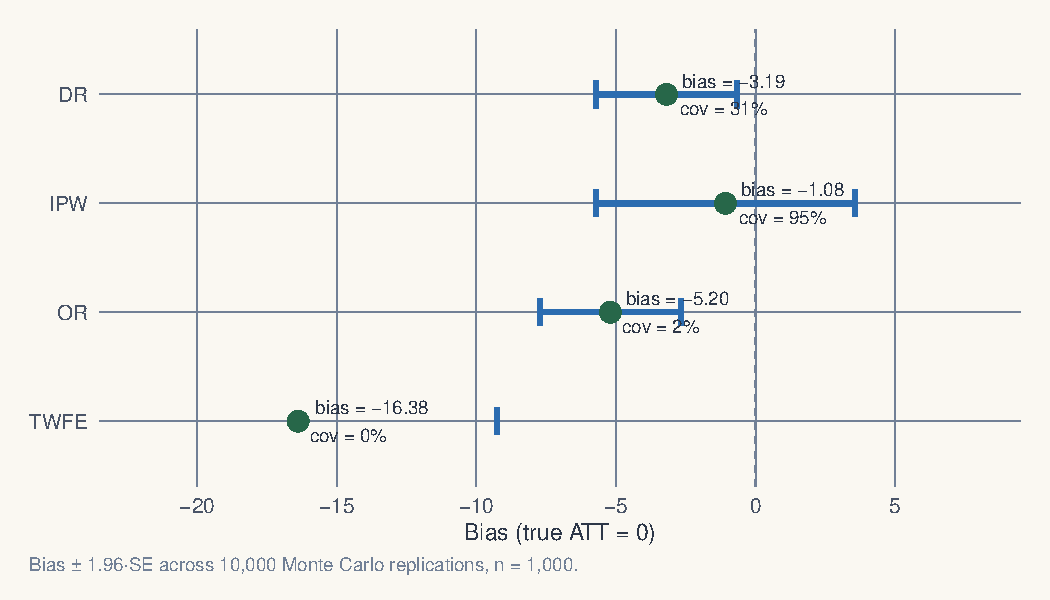
\includegraphics[width=0.68\textwidth]{figures/mc_dr_2.pdf}
\end{center}
\end{frame}

%% ----------
\begin{frame}{What the Monte Carlo teaches}
\vspace{0.8em}
\begin{itemize}\setlength\itemsep{0.55em}
  \item \textbf{TWFE + additive $X$:} coverage zero in every DGP. \highlight{Stop using it as a default.}
  \item \textbf{OR:} efficient when right. Coverage 1.5\% when wrong.
  \item \textbf{IPW:} less efficient, but robust to outcome misspecification.
  \item \textbf{DR:} best when one model is right. No better than IPW when both are wrong.
\end{itemize}
\end{frame}

%% ====================================================================
%% LALONDE APPLICATION
%% ====================================================================

\begin{frame}{Adding $X$ doesn't make your DiD credible}
\vspace{1.0em}
\begin{center}
\large
Adding $X$ shifts the credibility question---\\[0.6em]
from \highlight{``does PT hold?''}\\[0.5em]
to \highlight{``is my model of $Y(0)$ or $p(X)$ correct?''}\\[0.8em]
\color{warmgray}\normalsize
You still have to answer it.
\end{center}
\end{frame}

\begin{frame}{Now let's see it with real data}
\vspace{1.2em}
\begin{center}
\Large
LaLonde (1986) \textperiodcentered\ Dehejia \& Wahba (2002)
\end{center}
\vspace{0.8em}
\begin{center}
\color{warmgray}
A famous dataset where we \highlight{know the true effect.}\\[0.4em]
The benchmark: \highlight{\$1,794}.
\end{center}
\end{frame}

%% ----------
\begin{frame}{LaLonde (1986): the RCT found $\approx$\$800}
\vspace{0.8em}
\begin{itemize}\setlength\itemsep{0.6em}
  \item Job training program (National Supported Work Demonstration)
  \item Randomized --- treated and control groups assigned by lottery
  \item RCT estimate: earnings effect $\approx$ \textbf{\$800}
\end{itemize}
\vspace{0.6em}
\begin{center}\color{warmgray}\small
A clean causal estimate. The benchmark exists.
\end{center}
\end{frame}

%% ----------
\begin{frame}{LaLonde: dropped the RCT controls, used CPS instead}
\vspace{0.6em}
\begin{itemize}\setlength\itemsep{0.55em}
  \item Replaced the randomized controls with observational data (CPS, PSID)
  \item Re-ran every evaluator method from the literature
  \item Results ranged from \textbf{$-$\$16,000 to $+$\$3,000}
\end{itemize}
\vspace{0.5em}
\emphbox{The true effect was \$800. Not one method recovered it. \\
\textit{``The available evidence calls into serious question the ability of nonexperimental evaluators\ldots''}}
\vspace{0.3em}
\begin{center}\color{warmgray}\small
Empirical labor economics faces an evaluation problem.
\end{center}
\end{frame}

%% ----------
\begin{frame}{Dehejia \& Wahba (2002): propensity scores get close}
\vspace{0.6em}
\begin{itemize}\setlength\itemsep{0.55em}
  \item Need \textbf{two pre-treatment years} for all datasets --- uses a shorter sample
  \item RCT benchmark on this shorter sample: \highlight{\$1,794}
  \item Applied propensity score matching on the non-experimental sample
  \item Result: estimates close to \$1,794
\end{itemize}
\vspace{0.5em}
\begin{center}\color{warmgray}\small
Selective use of the data $+$ right method $=$ nearly recovered the truth.
\end{center}
\end{frame}

%% ----------
\begin{frame}{Our exercise: DiD with and without covariates}
\vspace{0.8em}
\begin{center}
NSW treated $+$ CPS controls \textperiodcentered\
Pre = 1975 \textperiodcentered\ Post = 1978\\[0.6em]
\large We know the effect: \highlight{\$1,794}\\[0.6em]
\normalsize\color{warmgray}
Let's see which specs recover it --- and which don't.
\end{center}
\end{frame}

%% ---------- Spec 0 ----------
\begin{frame}[fragile]{Naive TWFE: \$3,621 --- almost double the truth}
\vspace{0.4em}
\begin{lstlisting}[language=]
reg re i.post##i.ever_treated, robust
\end{lstlisting}
\vspace{0.5em}
\begin{center}
\begin{tabular}{lrr}
\toprule
Estimator & ATT & vs benchmark \\
\midrule
Naive TWFE & \textbf{\$3,621} & \textcolor{red}{$+$\$1,827} \\
\bottomrule
\end{tabular}
\end{center}
\vspace{0.4em}
\begin{center}\color{warmgray}\small
No covariates --- the CPS controls trend very differently from NSW treated.
\end{center}
\end{frame}

%% ---------- Spec A ----------
\begin{frame}[fragile]{Additive $X$: still \$3,621}
\vspace{0.4em}
\begin{lstlisting}[language=]
reg re i.post##i.ever_treated $X, robust
\end{lstlisting}
\vspace{0.5em}
\begin{center}
\begin{tabular}{lrr}
\toprule
Estimator & ATT & vs benchmark \\
\midrule
Additive $X$ & \textbf{\$3,621} & \textcolor{red}{$+$\$1,827} \\
\bottomrule
\end{tabular}
\end{center}
\vspace{0.4em}
\emphbox{Adding $X$ as time-invariant regressors does nothing here. The unit FE absorbs the level differences. The trend bias remains.}
\end{frame}

%% ---------- Spec B ----------
\begin{frame}[fragile]{Post$\,\times\,X$: \$1,711 --- now in the right range}
\vspace{0.4em}
\begin{lstlisting}[language=]
reg re i.post##i.ever_treated ///
    i.post##c.age i.post##c.agesq i.post##c.agecube ///
    i.post##c.educ i.post##c.educsq ///
    i.post##i.marr i.post##i.nodegree ///
    i.post##i.black i.post##i.hisp ///
    i.post##c.re74 i.post##i.u74, robust
\end{lstlisting}
\vspace{0.4em}
\begin{center}
\begin{tabular}{lrr}
\toprule
Estimator & ATT & vs benchmark \\
\midrule
Post$\,\times\,X$ & \textbf{\$1,711} & $-$\$83 \\
\bottomrule
\end{tabular}
\end{center}
\end{frame}

%% ---------- Spec C ----------
\begin{frame}[fragile]{Saturated TWFE: \$1,770}
\vspace{0.3em}
\begin{lstlisting}[language=]
* First-difference, then regress dy on X + D x X interactions
reg dy $X ///
    i.ever_treated#c.age i.ever_treated#c.agesq ///
    i.ever_treated#c.educ i.ever_treated#c.re74 ///
    i.ever_treated, robust
* Predict counterfactuals; ATT = mean(tau_sat) for treated
\end{lstlisting}
\vspace{0.3em}
\begin{center}
\begin{tabular}{lrr}
\toprule
Estimator & ATT & vs benchmark \\
\midrule
Saturated TWFE & \textbf{\$1,770} & $-$\$24 \\
\bottomrule
\end{tabular}
\end{center}
\end{frame}

%% ---------- OR ----------
\begin{frame}[fragile]{OR (HIT 1997): same answer as saturated TWFE}
\vspace{0.3em}
\begin{lstlisting}[language=]
* Fit trend model on controls only
reg dy $X if ever_treated == 0, robust
predict dy_hat
* ATT = mean gap for treated
gen delta_hat = dy - dy_hat if ever_treated == 1
\end{lstlisting}
\vspace{0.4em}
\begin{center}
\begin{tabular}{lrr}
\toprule
Estimator & ATT & vs benchmark \\
\midrule
OR by hand / \texttt{drdid reg} & \textbf{\$1,770} & $-$\$24 \\
\bottomrule
\end{tabular}
\end{center}
\vspace{0.2em}
\begin{center}\color{warmgray}\small
Saturated TWFE and OR are algebraically equivalent in the 2-period case.
\end{center}
\end{frame}

%% ---------- IPW ----------
\begin{frame}[fragile]{IPW (Abadie 2005): \$1,861}
\vspace{0.3em}
\begin{lstlisting}[language=]
drdid re $X, time(year) ivar(id) tr(ever_treated) ipw
\end{lstlisting}
\vspace{0.5em}
\begin{center}
\begin{tabular}{lrr}
\toprule
Estimator & ATT & vs benchmark \\
\midrule
IPW & \textbf{\$1,861} & $+$\$67 \\
\bottomrule
\end{tabular}
\end{center}
\end{frame}

%% ---------- DR ----------
\begin{frame}[fragile]{DR (Sant'Anna--Zhao 2020): \$1,979}
\vspace{0.3em}
\begin{lstlisting}[language=]
drdid re $X, time(year) ivar(id) tr(ever_treated) dripw
\end{lstlisting}
\vspace{0.5em}
\begin{center}
\begin{tabular}{lrr}
\toprule
Estimator & ATT & vs benchmark \\
\midrule
DR & \textbf{\$1,979} & $+$\$185 \\
\bottomrule
\end{tabular}
\end{center}
\end{frame}

%% ---------- Forest plot ----------
\begin{frame}{All seven estimators vs the \$1,794 benchmark}
\vspace{0.2em}
\begin{center}
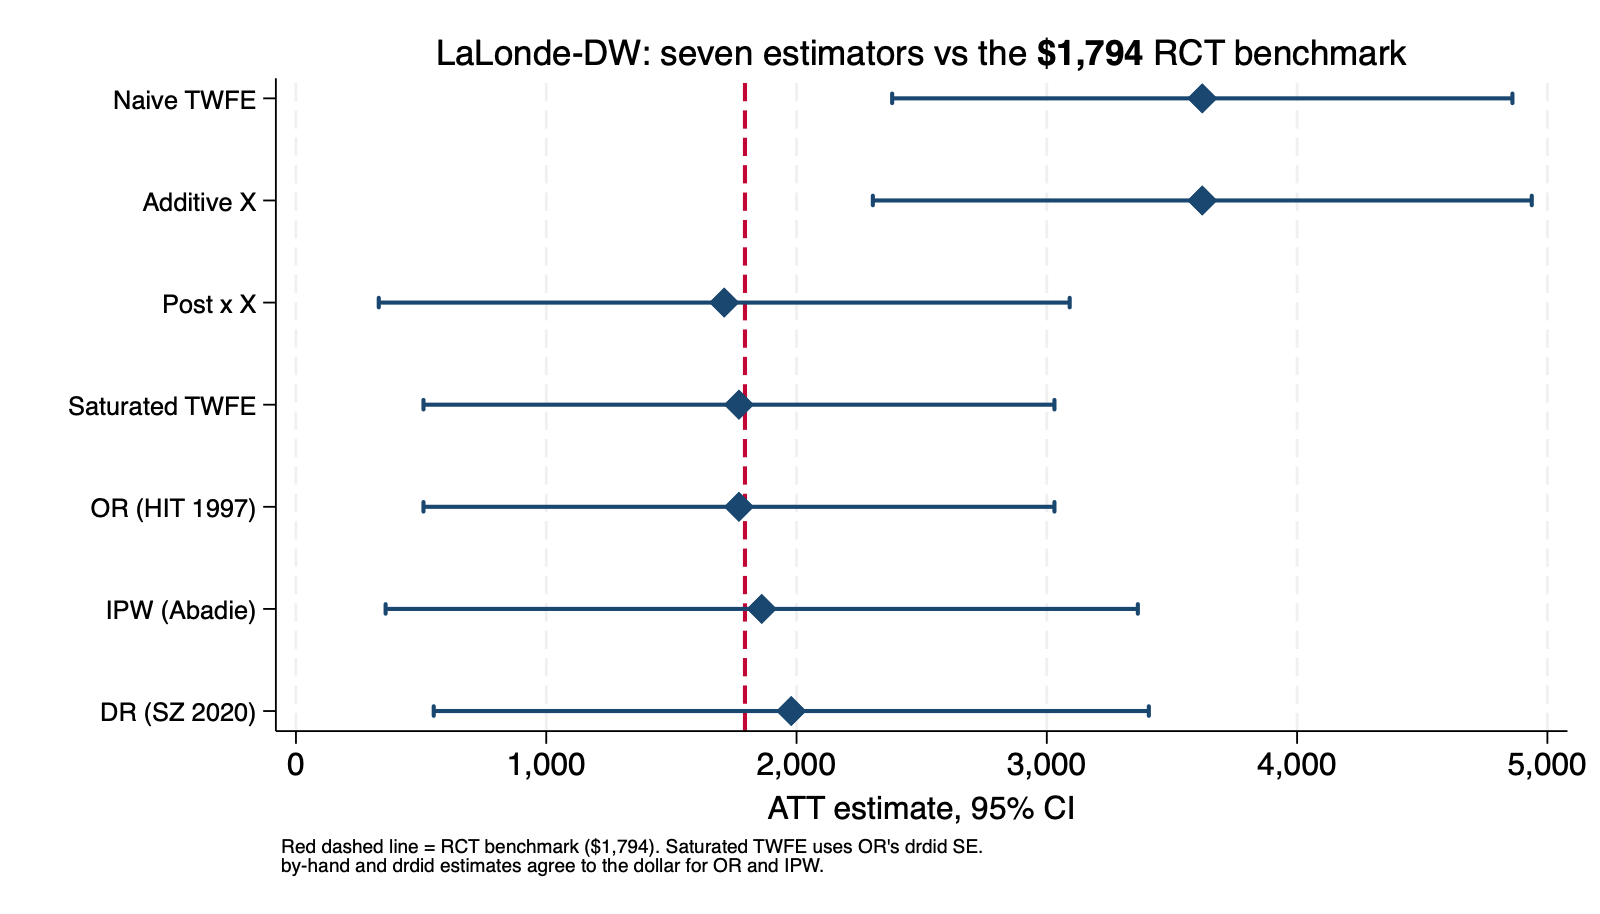
\includegraphics[width=0.82\textwidth]{figures/lalonde_forest.png}
\end{center}
\end{frame}

%% ---------- Conclusion ----------
\begin{frame}{Covariates are not robustness checks --- they are design}
\vspace{0.8em}
\begin{itemize}\setlength\itemsep{0.6em}
  \item People say: \textit{``if adding covariates changes results, be suspicious.''}
  \item That gets it backwards.
  \item We \highlight{know} the effect is \$1,794.
  \item Without covariates, or with additive covariates, we get \$3,621 --- \textit{wrong}.
  \item The correct specs recover \$1,770--\$1,979 --- \textit{right}.
\end{itemize}
\vspace{0.4em}
\emphbox{Covariates fix broken parallel trends. Changing your result is not a bug. It is the design working.}
\end{frame}

%% ---------- Closing linger ----------
\begin{frame}[plain]
\begin{tikzpicture}[remember picture,overlay]
\fill[cream] (current page.south west) rectangle (current page.north east);
\node[anchor=center, text width=0.84\paperwidth, align=center, text=charcoal]
  at (current page.center) {%
  \fontsize{18pt}{26pt}\selectfont
  The question is never\\[0.3em]
  {\color{accent}\bfseries ``did I control for $X$?''}\\[0.6em]
  The question is always\\[0.3em]
  {\color{accent}\bfseries ``did I get the model right?''}
};
\draw[accent, line width=1pt]
  ([yshift=1.4cm,xshift=0.25\paperwidth]current page.south west)
  -- ([yshift=1.4cm,xshift=-0.25\paperwidth]current page.south east);
\end{tikzpicture}
\end{frame}

\end{document}
